% !TEX root = ../main.tex
\chapter{Viphoger} \label{ch::viphoger}
\DndDropCapLine{A}{s a new nation, Viphoger is small. Its}
poleis are minuscule in comparison to the wilderness beyond, but their inhabitants live joyfully in their newly earned independence.

\begin{table*}[b]
\begin{DndTable}[width=\linewidth, header=Fagalian Calendar]{cXXX}
    \textbf{Month} & \textbf{Name} & \textbf{Tide} & \textbf{God} \\
    1              & Amion         & Blue          & Heliod, God of the Sun \\
    2              & Sianion       & Gold          & Ephara, God of the Polis \\
    3              & Granion       & Magenta       & Iroas, God of Victory \\
    4              & Zmivion       & Silver        & Phenax, God of Deception \\
    5              & Skenion       & Red           & Mogis, God of Slaughter \\
    6              & Danion        & Blue          & Kruphix, God of Horizons \\
    7              & Dibinion      & Gold          & Purphoros, God of the Forge \\
    8              & Ranion        & Magenta       & Athreos, God of Passage \\
    9              & Amelamion     & Silver        & Thassa, God of the Sea \\
    10             & Amelsion      & Red           & Erebos, God of the Dead \\
    11             & Amelgranion   & Blue          & Pharika, God of Affliction \\
    12             & Amelzvion     & Gold          & Nylea, God of the Hunt \\
    13             & Amelskenion   & Magenta       & Klothys, God of Destiny \\
    14             & Ameldanion    & Silver        & Karametra, God of Harvests \\
    15             & Ameldibinion  & Red           & Keranos, God of Storms \\
    16*            & Fisimmas      & White         & -
\end{DndTable}
\end{table*}
% * This day only occurs once every ten years.

Viphoger consists of a peninsula forming the south-western edge of the vast Whaler's Sea.
South from the sea, the land rises up to a ridge of mountains.
The lofty peaks of this ridge forms a barrier that few cross, so only rumors of the vast Dead Sea describe the land beyond.

To the west, the coastal lands become small pockets of forests crossed by a labyrinth of arid canyons, with the Zoedrem desert beyond.

The Siren's Inlet to the north is studded with islands large and small.
The largest cluster near the mainland, called the Dakra Isles, is poorly charted, and even those sailors who attempt to explore the isles return with contradictory information.
Eastward from Viphoger, the old nations of Yuadrem trade in the Whaler's Sea. % , regulated by the strong influence of the Seven Kingdoms of the Sea.

The heart of Viphoger lies in and around three poleis—cities and their surrounding territories.
Together the three poleis, Akhosh, Mephetis, and Setesh, encompass most of the population of Viphoger.
Mephetis covers the whole territory of the northeastern peninsula, Akhosh forms the frontier to the desert, and Setesh lies at the northern edge of the wild Nessian Wood.

The bands of the Uqhardu, the Vahagha, and the Pheres, roam the hills and badlands between the three poleis.
Remnants of the once great empire of Hulnar, now reduced to bandits and traders.
The mysterious leonin hunt in the valley of Oreskos, nestled between Mt. Kure and Winter's Heart.
Bughna gats and marsets dwell around the Stola Vale and the larger Nessian Wood.
And tortles live primarily in the coastal shallows of the Siren Inlet, though some manage to make comfortable homes among the gats of Mephetis.

The canyon of Katajthon, south of Akhosh, is the frontier where Akhoash soldiers clash with Treb gats.
Farther south-west is the city of Kofos, little known to Viphogerians.

The necropoleis of Asphodel and Odunos are home to the Returned --- zombie-like beings who have contracted the red pox.
Access to these lands is strictly forbidden, and is punishable by death in all three poleis.
The lands around these cities are bleak and barren, as if the Returned brought the pall of Nyx out with them into the mortal realm.

% !TEX root = ../main.tex
\subsection*{The Fagalian Calendar} \label{ssec::thefagaliancalendar}
The oth astronomers and philosophers from oldentimes established a calendar that has found massive adoption in the rest of Yuadrem.
It divides the year into fifteen months of twenty-four days, each beginning after the new Fagal.
Every ten years, an extra day is added at the end of the calendar to keep it aligned with the solar year.

The beginning of the year is considered the end of spring, so the new year begins with the summer.
Each month is associated to a tide, and is holy to a specific god.
A major festival in honor of that god is celebrated in Mephetis.
The fifth month (Skenion in Mephetis) is called Iroagonion in Akhosh, after the Iroan Games, which are held in that month every year.

% The Fagalian Calendar table summarizes the months, their lengths, and the god each is associated with.


% \incgraph[documentpaper,][width=\paperwidth,height=\paperheight]{02viphoger/img/00map.png}
% \newpage~\newpage

% !TEX root = ../main.tex
\subsection*{Life in the Poleis} \label{ssec::lifeinthepoleis}
Civilization in Viphoger is centered in three poleis: Akhosh, Mephetis, and Setesh.
These poleis exemplify the kins' drive to settle the land, to shape nature according to their needs, and to organize into political structures that can withstand the changing fortunes of the passing centuries.

Each polis is centered in a city but includes a wide region of surrounding territory, and each one has its own distinct society and culture.
To the people of Viphoger, ``Mephetis'' is more or less synonymous with ``Mephetians'' --- the polis isn't just the people who live in the city of Mephetis or even those who dwell in nearby villages; it is the people who follow the Mephetian way of life, wherever they might be found.

\subsubsection{Citizenship and Government}
In every polis, civic responsibility and full protection are afforded only to citizens.
Citizenship is limited to those whose parents were both citizens of the polis.
Citizens of other poleis, and their children, aren't permitted to participate in the government of the polis.
In Akhosh, citizens must meet one additional requirement: they must serve in the army.

The three poleis have different political structures, but each one has a council elected by popular vote of the citizenry.
The Twelve, Mephetis's council of philosophers, is the democratically elected ruling body of the polis.
Akhosh is ruled by a hereditary monarch who is advised by a council of elders elected by and from among the citizenry.
Similarly, Setesh's Ruling Council is formed by popular vote, and they govern the polis while its queen --- the goddess Karametra --- is absent.

\subsubsection{Trade and Currency}
Trade between Akhosh and Mephetis is constant and productive.
Caravans make the two-week journey between the poleis twice a month, aided by the Tsher river.
They carry fine Akhoshian metalwork and pottery to Mephetis, and Mephetian fabric, stonework, and fish westward.
Both poleis mint coins of copper, silver, and gold, with equivalent value.

Setesh trades with the other poleis as well, but less extensively.
Its Abora Market, just inside the city gates, is open to outsiders only on certain days, and Seteshan merchants prefer to barter goods rather than accept currency.
Despite these restrictions, Seteshan food, woodwork, and trained falcons are highly valued in the other poleis.

Aside from the other poleis, Mephetis and Setesh both trade with the dratl irds of the Vahagha band.
The irds don't work metal, so they trade woodwork, the produce of the plains, and woven blankets to the human poleis in exchange for weapons and armor.

\subsubsection{Recreation}
The people of the poleis enjoy the opportunity for some recreation, as time and money allow.

Gymnasia are popular gathering places, offering athletic training as well as space for philosophical discussion and friendly socializing.
A resident of the city might visit a gymnasium one day to exercise, the next to view a wrestling match between celebrated competitors, and the next to hear a renowned philosopher give a lecture on ethics.

Another important venue for recreation is the theater.
The works of celebrated playwrights, past and present, are regularly produced by casts of professional actors.
On occasion, a storyteller, accompanied by a small orchestra, draws crowds to a theater for a recitation of one of the great epics, such as The Sylvan Wars, The Theriad, or The Callapheia.
Such a performance might stretch over two or three days.

% !TEX root = ../main.tex
% \begin{tikzpicture}[remember picture,overlay]
%     \node[anchor=north, yshift=0.10cm] at (current page.north) {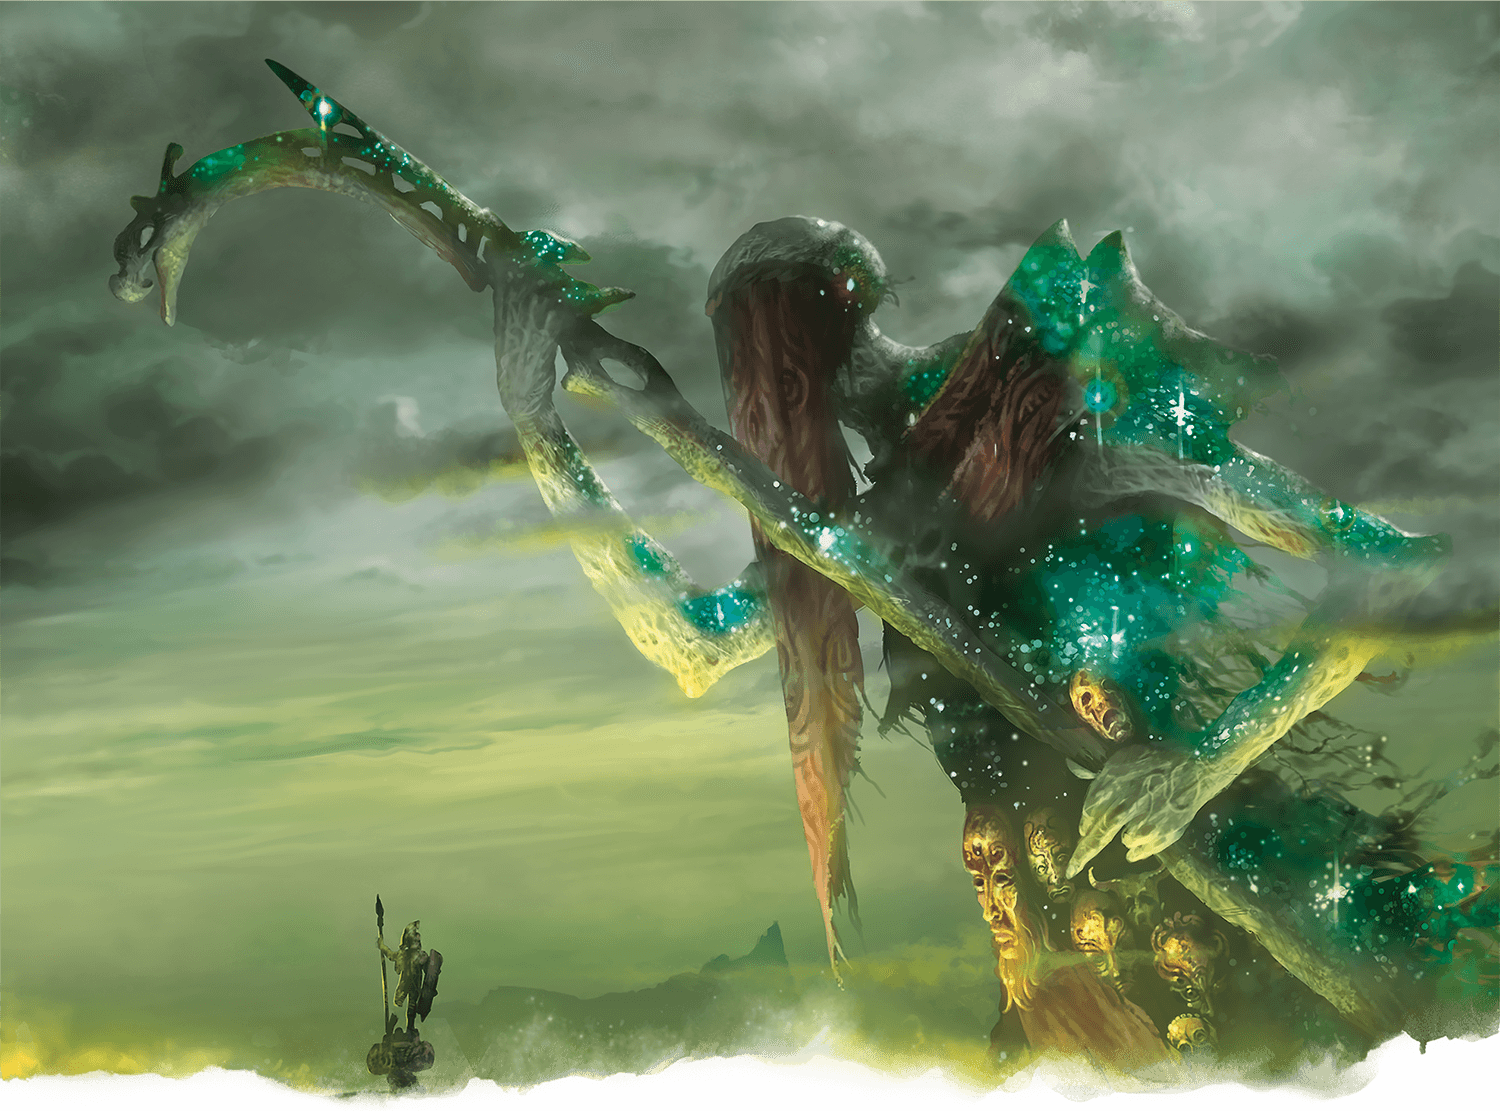
\includegraphics[width=\pdfpagewidth]{02viphoger/img/10athreos.png}};
% \end{tikzpicture}
%
% \vspace{14.0cm}

\section{Therism} \label{ssec::therism}

A pantheon of fifteen gods guides religious life on Viphoger.
From the sun and agriculture to death and passage into Nyx, the gods oversee the forces of nature and the most important aspects of mortal life.
These gods are quite real to the people of Viphoger, who see them moving across the sky at night and sometimes encounter them face to face.
Thus, most people perform rituals and devotions that honor various gods, hoping to win their favor and stave off their wrath.
They tell and retell the stories of the gods' deeds --- even as they watch those stories continue to play out in the vastness of the night sky.

Therism is the main religion practiced in Viphoger.
While both religions draw from the same pantheon, Tanethism and Therism couldn't have less in common.
The former was designed by a scholar and forced on their by a king, while the latter developed gradually from the gat settlers of the Sylvan Canyon.

In their new land, they saw the gods' visage in the sky, equating them to their ancient deities.
Not every mortal serves or acknowledges the gods, though.
Some philosophers in the schools of Mephetis teach that the gods of the pantheon are subordinate to a higher reality, perhaps the sky itself.
And other people, particularly leonin, believe that the gods are undeserving of mortal reverence.

\subsubsection{Worship}
    The most prevalent form of expressing reverence is the practice of libation, pouring out a splash of wine or water in honor of the gods.
    Pious people perform a simple rite of prayer and libation every morning and evening at a household altar or hearth, while the less devoted might still pour out a splash of wine before drinking the rest.

    The defining feature of a Theran temple is a statue of a god.
    Worshipers kneel before it, touch and kiss it, drape it in garlands and fine cloth, and leave offerings before it.
    % These acts are sometimes spontaneous outpourings of love or gratitude, and sometimes petitions, imploring the god to cure an illness, send rain for crops, guarantee a safe journey, or perform any other favor related to the god's sphere of influence.

    % Most people aren't devoted to a single god, though many prefer some gods over others. Someone might ask Pharika to spare a loved one from disease, then later offer prayers to Karametra for a bountiful harvest or to Thassa for safety on a sea journey.

    % Considering their significance to the people of Viphoger, this section includes a list of the 15 gods of the Therist pantheon, including a short description of each.

% !TEX root = ../main.tex
\subsection*{Athreos, God of Passage} \label{ssec::athreos}
    \subparagraph{Tides} Indigo, Silver.

    All mortals are destined to face Athreos, the River Guide, when their lives come to an end.
    The god of passage ferries the dead across the Tartyx River, conveying each mortal soul to its destiny in Nyx.
    For most people, Athreos embodies the greatest mysteries of existence --- the terror and wonder of life's last moment and the revelation of one's ultimate fate in the afterlife.
    % Athreos is no judge, though.
    The veiled, silent god undergoes no deliberations and makes no exceptions.
    The River Guide reads the truth of each soul and bears it unfailingly to its proper place in Nyx.
    There is no haggling and no sympathy on Athreos's skiff, the god having heard and denied every mortal plea.

    Athreos appears as a gaunt figure cloaked in ragged robes and a collection of golden masks.
    What little can be seen of their body is unsettling, its gray flesh stretched thin over a barely et skeleton.
    The River Guide is never without their ancient staff, Katabasis, which they transforms into the ferryboat they use to ply the Rivers That Ring the World.
    Athreos can change shape but rarely, if ever, takes on other forms.

    % \begin{figure}[t]
    %     \centering
    %     
\includegraphics[width=0.47\textwidth]{02viphoger/img/10s_athreos.png}
    % \end{figure}

    \subsubsection{Worshiping Athreos}
        Most funeral traditions include small offerings and words of reverence to Athreos.
        Predominant among these traditions is burying or burning the dead with a clay funerary mask, to ``frame'' the identity of the dead for Athreos, and with at least one coin, so a soul might pay Athreos to ferry them to Nyx.
        % Some people are laid to rest with large amounts of grave goods.
        Memorial practices vary widely by culture, from tearful, somber affairs to lively celebrations.
        These rituals serve more as catharsis for the living than as meaningful boons to Athreos, though.
        The River Guide cares only for the single coin they're owed by any who board their skiff.

        During the feast of Necrologion, pious souls silently spend the day reading ancient memoirs or writing messages for their own descendants.
\subsection*{Ephara, God of the Polis} \label{ssec::ephara}
    \subparagraph{Domains} Indigo, Blue.

    As god of the polis, Ephara sees themself as the founder of civilization.
    They watch over cities, protecting them from outside threats.
    They are credited with establishing the first code of law, which Mephetis has preserved and the other poleis have imitated.
    Even more important, they help cities reach their highest potential, becoming centers of scholarship, industry, and art.

    Ephara appears as a huge animated statue wearing a stone crown, resembling the capital of a column.
    When they choose to walk about their cities at a mortal's scale, they often take on the form of a gat.
    In either form, they are always dressed in blue and white, and their expression is usually serious, but not unkind.
    They often carry a large urn on one shoulder, with the dark, star-studded sky pouring from it and dissolving into mist as it hits the ground.

    % \begin{figure}[b]
    %     \centering
    %     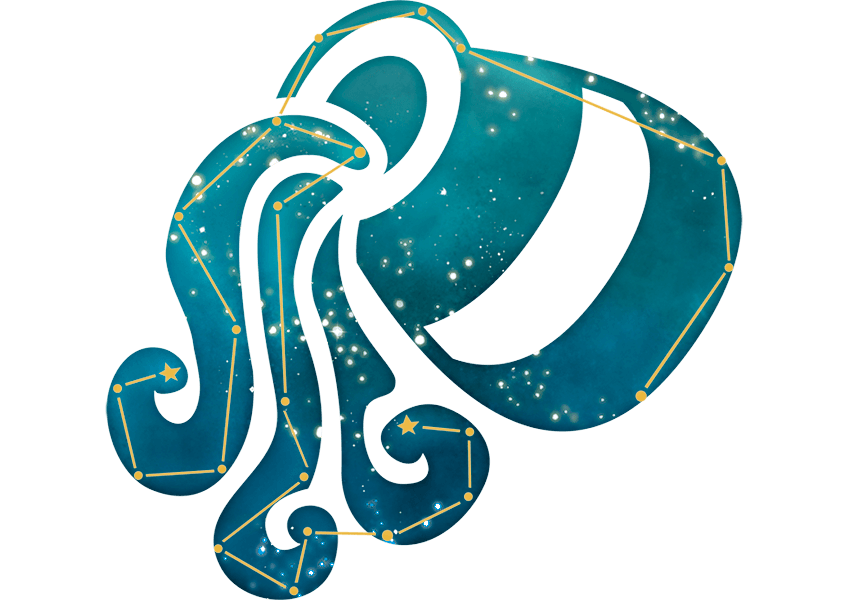
\includegraphics[width=0.47\textwidth]{02viphoger/img/10s_ephara.png}
    % \end{figure}

    \subsubsection{Worshiping Ephara}
        To an extent, Ephara's devout show their faith by going about their lives and contributing to society.
        Midday services at Ephara's temples often feature a brief prayer, followed by a longer talk from an industrial or civic leader on a topic of general interest.
        Attendants often bring meals to eat while on a break from their jobs.

        Ephara's face is a common sight in cities.
        Marble buildings, stone walls, and similar surfaces usually feature a sculpture or relief of their visage.
        People often swear oaths or engage in verbal disputes in front of these images, believing they won't let a falsehood told in front of them go unpunished.
        Whether they actually intervenes is unclear, but conflicts that play out this way are often resolved peacefully, without a need for the justice system to get involved.

\subsection*{Erebos, God of the Dead} \label{ssec::erebos}
    \subparagraph{Domains} Silver.

    Erebos is the god of death and Nyx, lord of all that has ever lived.
    % They preside over the bitterness, envy, and eventual acceptance of those who suffer misfortune.
    Their hoarding of both souls and the treasures the dead carry into Nyx see them worshiped by those who desire to collect and keep wealth.

    Erebos's very presence is stifling, and those who come face to face with them often depart in despair.
    They are jealous and tyrannical within their realm, but unlike their brother Heliod, they neither bluster nor try to expand their influence.
    They wait patiently, secure in the knowledge that everything belongs to then in the end.

    Erebos most frequently appears as a slender, gray-skinned gat with two large, outward-curving horns, wielding a long black whip.
    They also appear in the form of a black asp, a cloud of choking smoke, or an animated golden idol.

    % \begin{figure}[b]
    %     \centering
    %     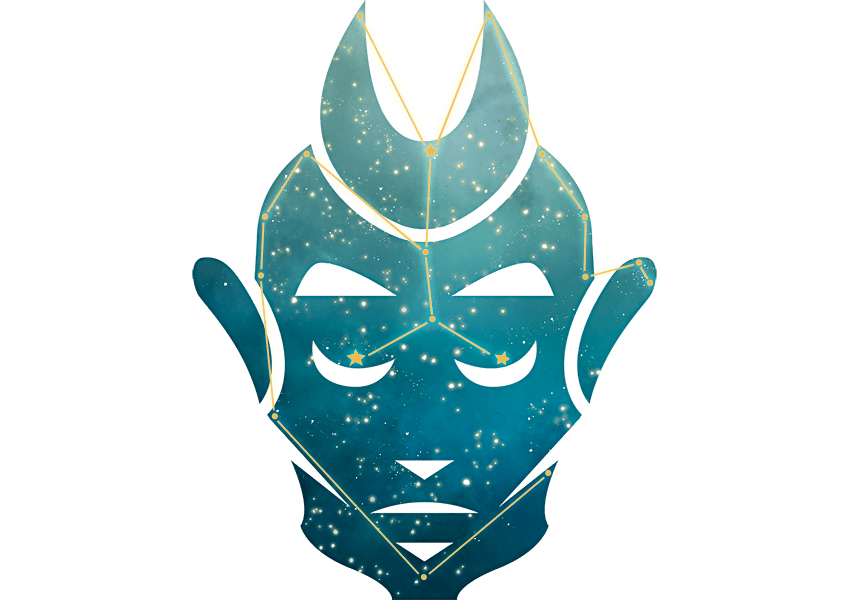
\includegraphics[width=0.47\textwidth]{02viphoger/img/10s_erebos.png}
    % \end{figure}

    \subsubsection{Worshiping Erebos}
        To many mortals, Erebos is primarily concerned not with death, but with gold.
        Most of their followers downplay their association with death and misfortune, praying to them for material wealth.
        Others pray to them because they want to be more accepting of their misfortune.
        These individuals see themselves as beyond hope, asking only that Erebos grant them the strength to endure until they enter their realm at their predestined time.

        A smaller but more dangerous group of Erebos worshipers are those who glorify death.
        These cultists and assassins congregate in secret in communities across Viphoger, engaging in campaigns of violence.

        The only major festival dedicated to Erebos is the Katabasion or ``the Descent'', features a ceremony in which worshipers make a symbolic journey into Nyx.
        The supplicants enter a cave, offer prayers and sacrifices to Erebos in utter darkness, and slowly make their way back to the surface just before sunrise.

% !TEX root = ../main.tex
\subsection*{Heliod, God of the Sun} \label{ssec::heliod}
    \subparagraph{Domains} Light.

    Heliod is the radiant god of the sun.
    According to myth, they ensure that the sun rises every day to provide light and warmth to the world.
    Every inhabitant of Viphoger acknowledges their dominant presence, and nearly everyone at least pays lip service to the idea of giving them worship and honor.

    Pride and self-assurance radiate from Heliod as light floods from the sun.
    They are cheerful and sociable, enjoying the company of others and forming bonds easily.
    Their friendship can be as easily lost, though, turning them from ally to enemy as the consequence of a single misstep or perceived betrayal.

    Heliod has appeared to mortals in a variety of forms, but they prefers the appearance of a sun-bronzed gat in their forties, dressed in a flowing tunic of golden cloth.
    Their profile is noble, highlighted by a strong chin and a short beard, and they boast the broad chest of a perfectly fit athlete.
    Their hair is glossy black, and their head is crowned with a golden wreath.
    They are also fond of appearing as a brilliant white horse or a radiant golden stag.
    In any guise, they look lit by the sun, even when they travel across the night sky.

    \subsubsection{Worshiping Heliod}
        The brilliance of Heliod's sun is impossible to ignore.
        Thus, virtually everyone on Viphoger pays at least grudging respect to the sun god in forms of worship that range from simple gestures to days-long celebrations.

        Some families, particularly in the polis of Mephetis, follow a practice of bowing in the direction of dawn's first light --- or winking, in a gesture of respect for the sun god's luminous ``eye''.
        More dedicated worshipers offer short litanies at dawn, noon, and dusk, acknowledging the sun's passage across the sky.

\subsection*{Iroas, God of Victory} \label{ssec::iroas}
    \subparagraph{Domains} War.

    Iroas is the steadfast god of honor and victory in war.
    When soldiers march to battle, their voice is the thunder of their footsteps and the crash of spear on shield.
    Soldiers, mercenaries, and athletes all pray for Iroas's favor in securing victory.
    Common folk pray to Iroas for courage and fortitude in times of struggle, for their is the battle nobly fought and won.

    Bold and confident with a soldier's demeanor, Iroas is the pinnacle of martial pride and bearing.
    They are stoic almost to a fault, but also exhibits a wry sense of humor.
    Those who honorably shed blood in Iroas's name can count on their support.
    Cowards and oath breakers are to be despised, and traitors don't deserve mercy in battle.

    Iroas most often appears as a powerfully built gat with a bull-like body, clad in gleaming armor and wielding a spear and shield.
    They speak in a booming baritone that projects power, confidence, and courage.
    They have been known to appear as a burly soldier or a mighty bull before their followers.
    Whatever form they choose, Iroas carries themself with precision and majesty at all times and doesn't tolerate disrespect or undue informality from those who would deal with them.

    \subsubsection{Worshiping Iroas}
        Iroas is interested not in pretty words, but in great deeds.
        The faithful of Iroas show their piety by comporting themselves well in contests of athleticism or skill.
        Swearing an oath to win a battle in Iroas's name and failing to do so is a great shame upon a warrior, thus such a promise is never uttered lightly.

        The fifth month of the Fagalian calendar is Skenion, named for an annual commemoration of the Mephetian conquest of Natumas.
        This victory cemented Mephetis's control over the entire peninsula.
        But in Akhosh, the month is called Iroagonion, for the Iroan Games.
        These games are the grandest display to honor Iroas.
        To even compete in the Iroan Games is considered noteworthy, as the poleis send only their finest athletes.
        The grand prize, besides a ceremonial wreath, is the opportunity to be visited by Iroas themself.

\subsection*{Karametra, God of Harvests} \label{ssec::karametra}
    \subparagraph{Domains} Life, Nature.

    Karametra is recognized as the serene, maternal god of the harvest, her arms spread wide as she offers bounty to her worshipers or cradles communities in her embrace.
    Almost every uman settlement contains at least a modest shrine to solicit her favor, and she is closely associated with Setesh, the center of her worship.

    Wise and even-tempered, Karametra values community, stability, and the balance of nature.
    She is the god of maternity, family, orphans, domestication, and agriculture, as well as defense of the home and territory.

    Karametra appears to mortals as a motherly figure with hair made of ordered rows of leaves that shroud her eyes from view.
    She is always shown in art (and often seen in the night sky) seated on her throne, which is formed from a tangle of grape vines growing out of a collection of jugs and amphorae that surround her.
    An elaborately carved wooden canopy extends above her, and a giant sable --- her faithful companion --- curls around the base of the throne at her feet.
    In one hand, she holds a harvester's scythe.

    \subsubsection{Worshiping Karametra}
        The earth's fertility is essential for mortal life to continue.
        Those who live in the modern poleis might not be as aware of that fact as those who farm their own food, but even they long for children, know the pinch of hunger, and feel the turn of the seasons.

        Prayers to Karametra focus on asserting Karametra's constancy and bounty, praising the god's love and generosity.
        Worshipers of Karametra gather for a feast once a month, on the evening of the full Fagal, that celebrates the god's role in parenthood and community.
        New parents receive gifts and blessings, and young couples sneak away into the woods in hopes of finding sweet berries and sweeter kisses.

% !TEX root = ../main.tex
\subsection*{Keranos, God of Storms} \label{ssec::keranos}
    \subparagraph{Domains} Knowledge, Tempest.

    Keranos is the god of storms and wisdom.
    Merciless and impatient, Keranos is equally likely to strike out at mortals with a bolt of inspiration or a blast of lightning.
    To revere Keranos is to exult in the power of wisdom, clarity of purpose, and the fury of the storm.
    They are favored by tinkerers, inventors, and sailors as well as those seeking solutions to intractable problems.
    They don't tolerate the company (or the worship) of fools, and they despise vapidity and indecision.

    Keranos rarely appears directly to mortals, preferring to communicate through an epiphany or a crashing bolt of lightning.
    When they do deign to manifest in the mortal world, Keranos prefers the form of a stout, bearded, gat wearing a purple loincloth girdled in a steel chain belt with a clasp in the form of a wyvern's skull.
    Their bearing is upright and stern, with a clipped, brusque way of speaking.
    Particularly clever plans and observations bring a hint of a smile to their face.
    When interacting with mortals, Keranos sometimes appears in the form of a great horned owl with lightning strikes flashing in its eyes.

    \subsubsection{Worshiping Keranos}
        Keranos's name is often invoked by those amid a storm who seek safety, or by someone who is faced with a particularly difficult problem.
        Only the foolhardy call out to Keranos frivolously or in jest, since they might well smite the offender with a bolt from the blue.

        In Akhosh, where Prince Cymede actively promoted the worship of Keranos, elaborate ceremonies are conducted beginning just before the first summer thunderstorm.
        Intricate, open-framed sand paintings with complex geometric shapes are created by dancers in flowing blue silken wraps.
        Then, as the rains fall, the paintings are washed away, symbolizing the impermanence of genius and the power of change.
        Akhoash oracles strive to predict the exact time of the first storm in hopes of allowing enough time to stage the celebration.
        A similar festival in Mephetis, called the Astrapion (``Lightning Festival''), happens during the third month of the year.

        On the last day of every month, Keranos's priests and laity bring offerings of fish and distilled spirits to their temples.
        The fish are cooked under a skylight open to the stars, with a shot of spirits thrown on the fire.

\subsection*{Klothys, God of Destiny} \label{ssec::klothys}
    \subparagraph{Domains} Knowledge, War.

    Believed to have sprung into existence during Yuadrem's earliest days, Klothys is the god of destiny and, along with Kruphix, one of the world's original deities.
    They oversee the order of the cosmos, ensuring that all things remain in their proper place, knowing how easily the cosmic balance could be undone if they were not vigilant.
    On the heels of a near-catastrophic upset of the cosmic order --- the rise to godhood and subsequent defeat of the gat Xenagos --- Klothys has emerged from the Underworld for the first time in mortal memory to untangle the strands of destiny and set the world right.

    Klothys typically appears as a gat with six curling horns and an impossibly long mane of pale hair that cascades around their horns, drapes over their eyes, and spools into their spear-like weapon and the various other spindles they carry.

    Beneath their outward calm, Klothys seethes at the way mortals and gods alike have pulled apart and rearranged the threads of destiny to feed their petty ambitions.
    Their peaceful mien falls away in the presence of such villains.
    In their rage, their red-glowing eyes come into view through the veil of their hair, and they wield burning strands of hair as a devastating weapon.

    \subsubsection{Worshiping Klothys}
        Klothys doesn't trace their origins to mortal devotion, and they have languished in obscurity for almost the whole of Viphoger's history.
        They don't need worship to sustain or empower them, and they don't seek out reverence or demand it.
        By and large, mortals are irrelevant to them, except insofar as they have played a role in tangling the strands of destiny by defying nature's order.

\subsection*{Kruphix, God of Horizons} \label{ssec::kruphix}
    \subparagraph{Domains} Knowledge, Trickery.

    Kruphix is the enigmatic god of mysteries, horizons, and the passage of time.
    Their followers claim that they know not only everything that is known at present, but everything that has ever been known by anyone.

    Quiet surrounds Kruphix like a shroud.
    Standing apart from the other gods, they speak rarely, even to their most favored followers.
    When they do communicate, it is often as a barely audible whisper.
    Kruphix can speak with a booming voice directly into the minds of all the other gods simultaneously, though, doing so when something threatens the cosmic order.

    Kruphix's true form is more abstract than that of any of the other gods.
    They appear only in star-filled silhouette, usually as a hooded, four-armed figure of indeterminate species and gender.
    Two of the stars in their ``body'' often shine brightly, suggesting eyes.
    Kruphix's starry silhouette sometimes takes the form of a bird or a whale.

    \subsubsection{Worshiping Kruphix}
        Many pray to Kruphix when they need to find something lost, but few dedicate themselves to their worship.
        Cults devoted to Kruphix fiercely guard their secrets, and their initiates refrain from drawing attention to themselves.
        Some followers and champions of Kruphix travel the world in secret, searching for hidden truths.
        Many use secret signals to enable them to find safe lodging with other worshipers nearly anywhere.

        Rituals honoring Kruphix are usually performed at boundaries, both temporal and spatial: shorelines, riverbanks, equinoxes, and sunsets.
        One of the god's greatest festivals is the Agrypnion (``The Watching''), which marks the end of summer and the close of the year.

% !TEX root = ../main.tex
\begin{tikzpicture}[remember picture,overlay]
    \node[anchor=north, yshift=0.10cm] at (current page.north) {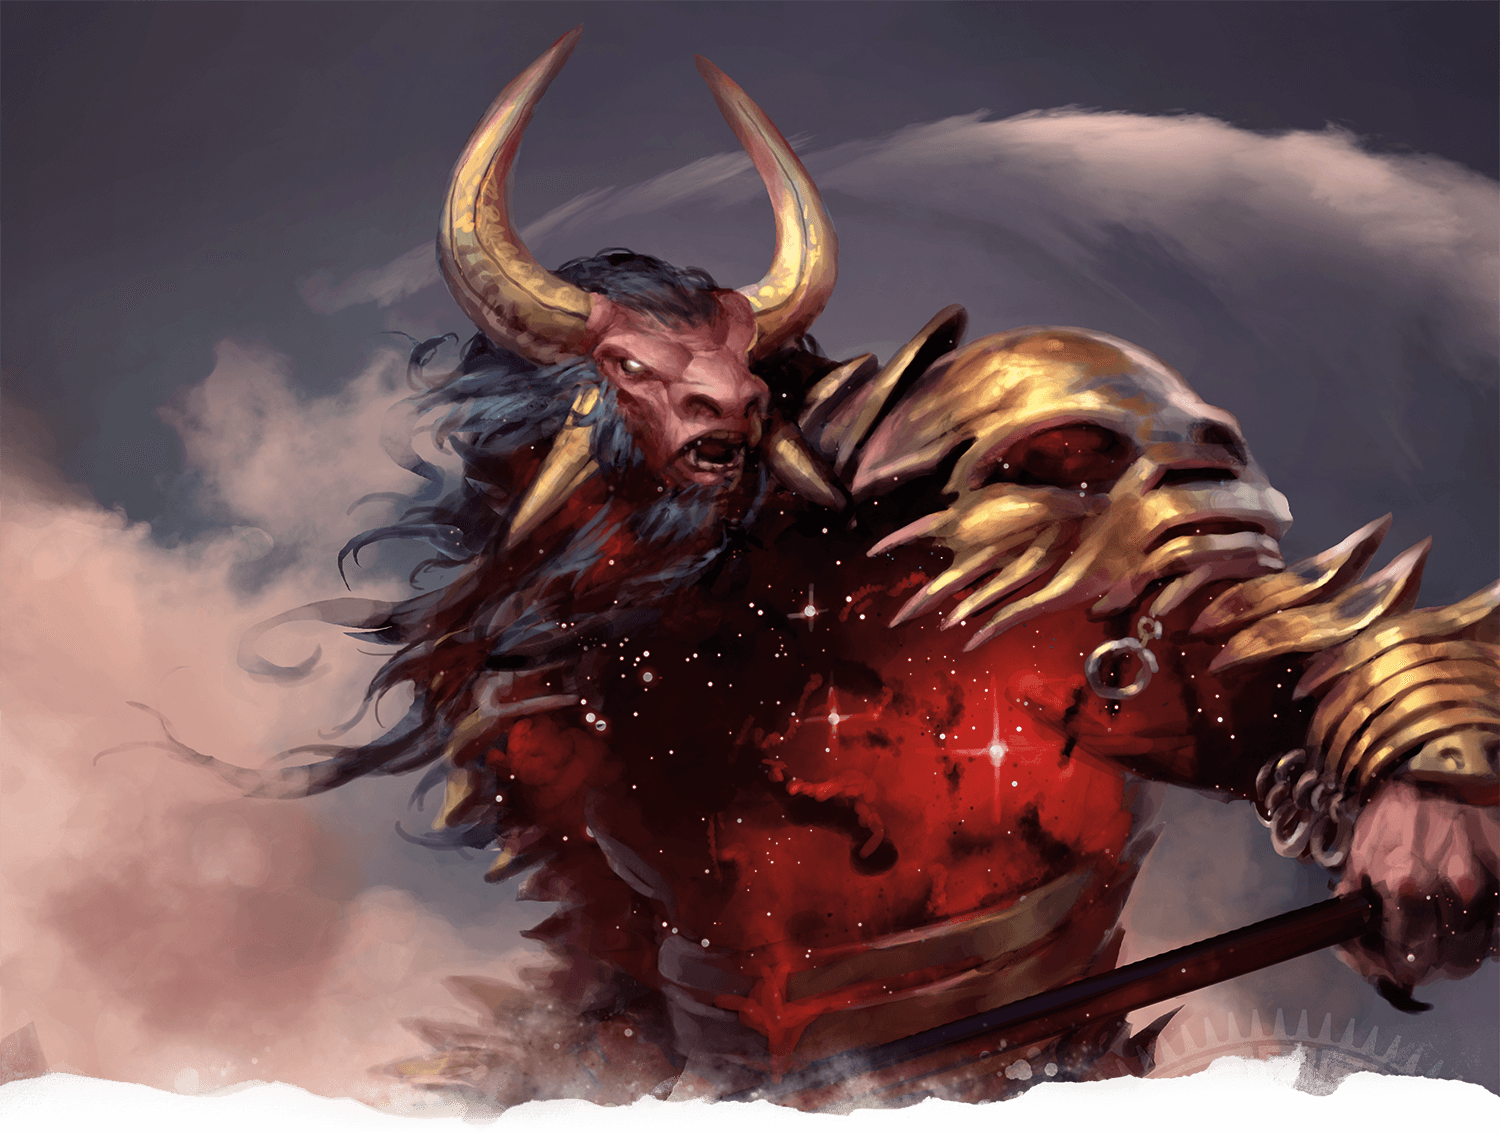
\includegraphics[width=\pdfpagewidth]{02viphoger/img/10mogis.png}};
\end{tikzpicture}

\vspace{13.5cm}

\subsection*{Mogis, God of Slaughter} \label{ssec::mogis}
    \subparagraph{Domains} War.

    Mogis is the god of slaughter, violence, and war.
    They are hatred unrestrained, empathy denied, and mercy forgotten, an entity whose very presence incites mortals to violence.
    Soldiers fear succumbing to their blood lust lest they dishonor themselves, but the vengeful and forsaken call to Mogis for the gift of their rage.
    They are the sibling of Iroas, god of victory, and their antithesis in matters of warfare.

    % The anger and malice radiating from Mogis is almost palpable.
    % They exercise no control over their temper or their urges and lash out at subordinates at the slightest provocation.
    % Akhoash soldiers are warned that to give in to their seductive battle rage is to risk becoming an androphage --- a bloodthirsty killer wholly consumed by Mogis's fury.

    Mogis cuts a terrifying figure, appearing as a four-horned treb gat of incredible size clad in spiked bronze armor and wielding a massive ebon greataxe.
    They don't debase themself by appearing in other guises to mortals --- to behold them is to behold the cruelty of war personified.
    They hunger endlessly to defeat their brother Iroas in combat and thus become the sole avatar of war among mortals.

    \begin{figure}[b]
        \centering
        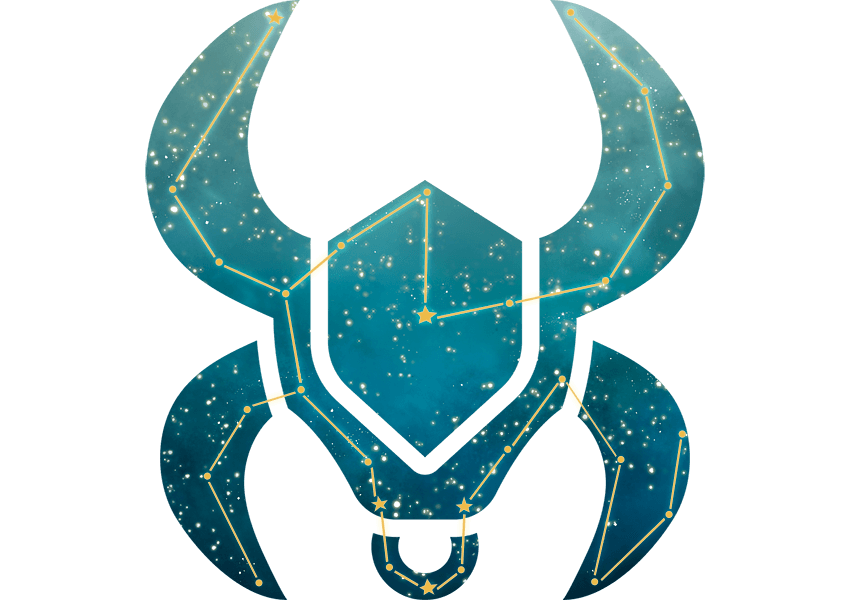
\includegraphics[width=0.47\textwidth]{02viphoger/img/10s_mogis.png}
    \end{figure}

    \pagebreak~
    \vspace{14.0cm}

    \subsubsection{Worshiping Mogis}
        Mogis exhorts their followers to channel their hatred and rage into ever greater acts of cruelty and violence.
        They demand actions over words, making their followers a dangerous lot.
        From the spurned lover thirsting for revenge to the blood-drenched warrior on the battlefield, all honor Mogis with the shedding of blood in anger.

        % Treb gats are the most ardent worshipers of Mogis and regularly hold bloody rites in their honor.
        % Warchanters, the clergy of Mogis, whip their marauders into a near-mindless frenzy before battle; the ensuing slaughter gives glory to Mogis's name.

        % The appearance of a blood moon is a most holy occasion for the faithful of Mogis, since the moon represents their hateful crimson eye.
        % At such times, their followers prepare and consume a feast of meat, either raw or barely cooked, along with copious amounts of intoxicants, followed by ritual self-mutilation --- scarring themselves to demonstrate their devotion to Mogis.

\subsection*{Nylea, God of the Hunt} \label{ssec::nylea}
    \subparagraph{Domains} Nature.

    Nylea is the wild, carefree god of the hunt.
    They claim dominion over the whole of the natural world, particularly hunger and predation, the seasons, metamorphosis and rebirth, and the forest.

    Nylea is among the most gregarious of the gods, and can be spotted frolicking joyfully with their Nyxborn lynx, Halma, or their favorite nymph, Theophilia.
    But they also savor solitude, and on the hunt they are deadly serious, almost animalistic, in their mood.
    They are nearly as quick to anger as their sibling Purphoros, enacting swift revenge on those who harm the natural realm.

    Nylea usually appears as a green-skinned dryad with woody extremities.
    Their hair is made of vines and leaves that change with the seasons.
    They might also appear as a majestic specimen of any animal, most frequently a lynx or a wolf.
    When they desire stealth or solitude, they might take the form of a tree, usually an oak or an olive.

    \begin{figure}[b]
        \centering
        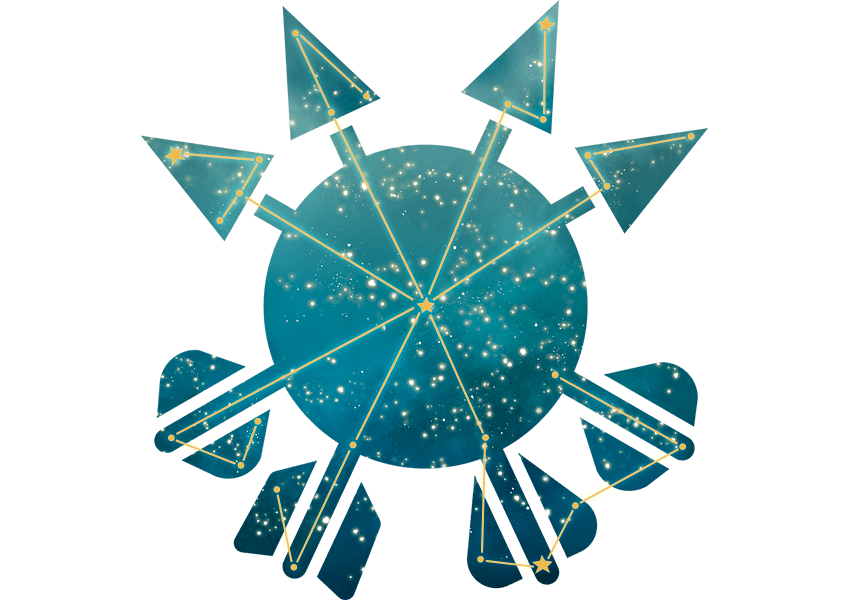
\includegraphics[width=0.47\textwidth]{02viphoger/img/10s_nylea.png}
    \end{figure}

    \subsubsection{Worshiping Nylea}
        Mortals all over Viphoger pray to Nylea when they rely on hunting or nature's whims for their livelihood.
        Their most ardent followers are bughna gats and humans (particularly those who live in Setesh and in the wilds), and nymphs of all kinds, especially dryads.
        Few leonin worship any of the gods, but of those who do, many favor Nylea with their prayers.

        Nylea blesses those who are kind to animals, considering such acts as wordless prayers.
        Those who must kill a dangerous natural animal or cut down trees often pray to Nylea for forgiveness, sometimes leaving food for other animals or planting new trees as atonement.

\pagebreak

\subsection*{Pharika, God of Affliction} \label{ssec::pharika}
    \subparagraph{Domains} Death, Knowledge, Life.

    Pharika is a god of affliction and medicine, alchemy and aging.
    % In the earliest days of the Sylvan Canyon, Pharika seeded the world with countless secret truths --- mysteries of medicine, minerals with strange properties, nexuses of magic, and the like --- which they hid among Nylea's wilds and the shadows of Erebos's Nyx, leaving clues where mortals might find them.
    It isn't altruism that drives them; they study the innovation and suffering of mortals, deciphering in them ever greater mysteries as they treat Viphoger as their personal laboratory.

    Pharika typically takes the form of a qulbaba ird with the lower body of a snake, similar to a couatl.
    Their body is thickly scaled and a pair of bronze-scaled vipers seamlessly emerge from their chest.
    They are never without their kylix, a drinking cup within which they can produce virtually any medicine or toxin.
    When their aims require subtlety, Pharika often takes the form of a serpent, or sometimes an aged gat.

    % Little escapes Pharika's cool gaze.
    % Even when outwardly friendly, they are cunning and calculating, watching for the slightest sign of weakness or desire that they can exploit later.
    % Those who offend them rarely recognize their misstep until they strike.

    \begin{figure}[t]
        \centering
        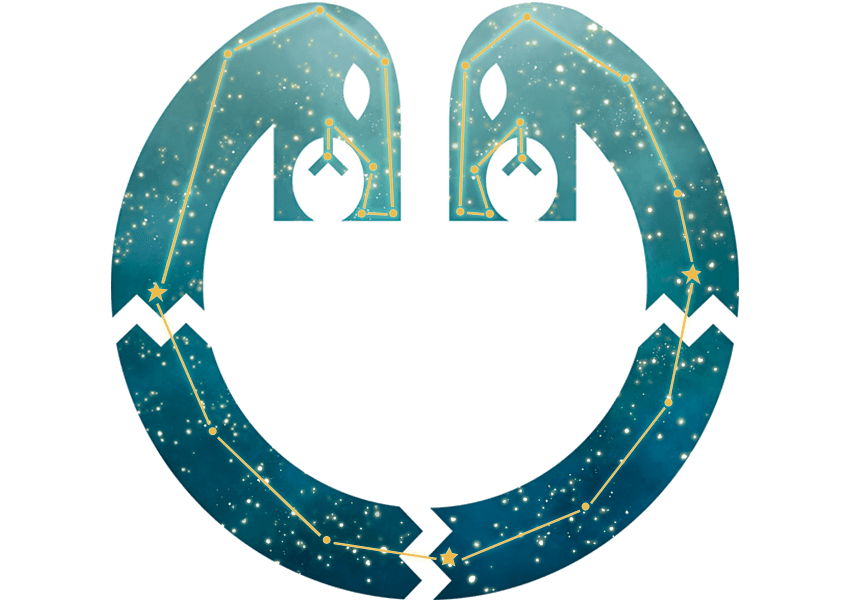
\includegraphics[width=0.47\textwidth]{02viphoger/img/10s_pharika.png}
    \end{figure}

    \subsubsection{Worshiping Pharika}
        The diseased and the dying alike often make written entreaties to Pharika for a remedy.
        Prayers are written on scraps of paper or shards of pottery, sealed in small pots, and buried in bogs, leaving them as secrets for others to exhume years later.
        Many people pray to them before undergoing a medical procedure, picking herbs, or confronting a venomous animal.
        Nights of a waxing crescent Nuagal (from the 10th to the 18th of Amion, Zmivion, Dibinion, Amelsion, and Amelskenion, when a sliver of Nuagal lingers in the early evening) are sacred to Pharika and are thought to be an auspicious time to harvest medicinal plants.

        Pharika's followers include members of several small mystery cults, which embrace varying aspects of their divine nature.
        The most infamous of these is the Cult of Frozen Faith, led by a lampad.
        Initiates receive a lethal dose of poison, become petrified, and then are restored to flesh one year later.
        Petitioners who have Pharika's favor emerge alive and healthy; those they doesn't care for fail to survive the transformation.

% !TEX root = ../main.tex
\subsection*{Phenax, God of Deception} \label{ssec::phenax}
    \subparagraph{Domains} Blue, Silver.

    Phenax is the masked patron of lies and cheats.
    They are Heliod's ethical antithesis, governing the spheres of gambling, deception, and betrayal.
    Phenax was once a mortal who was trapped in Nyx, but they learned how to forsake their identity to prevent Erebos from detecting what they were doing.
    They crossed back over the Rivers That Ring the World wrapped in the tattered cloak of Athreos, the River Guide.
    Hidden by illusion as they were, neither Athreos nor Erebos could find Phenax and bring them back.

    % Able to play whatever role the situation calls for, Phenax is a consummate actor.
    % Their incisive wit and cunning enable them to read the desires of their marks, adjusting their approach to suit the moment.
    % In their rare moments of candor, Phenax is calm and calculating, always looking toward their next scheme.

    Phenax is a shadowy and mysterious figure.
    When appearing before mortals, they prefer the form of a willowy gat with ashen gray skin, clad in elegant robes.
    They have also been known to appear in a variety of animal forms, including the shapes of asps, mockingbirds, or rats.
    Regardless of their shape, a mask forever conceals the blank face of the first Returned.

    % \begin{figure}[t]
    %     \centering
    %     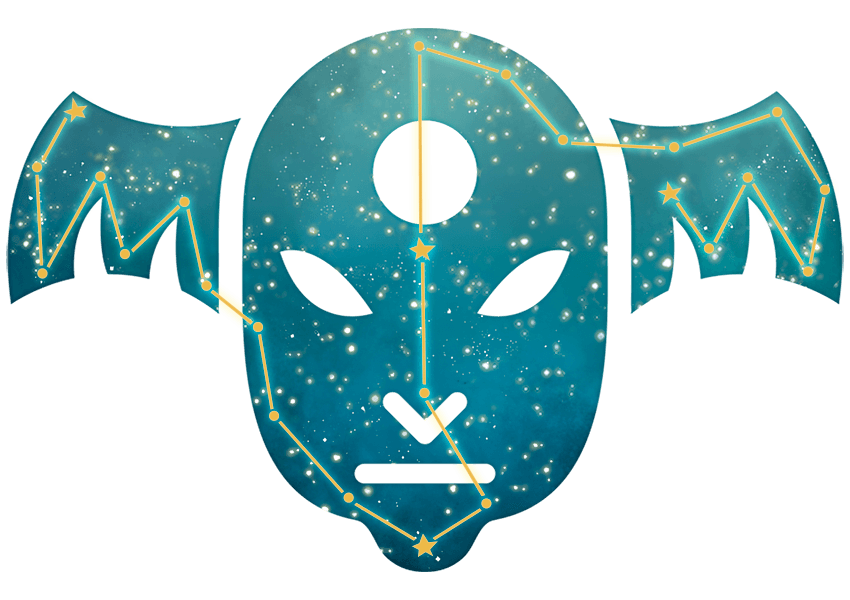
\includegraphics[width=0.47\textwidth]{02viphoger/img/10s_phenax.png}
    % \end{figure}

    \subsubsection{Worshiping Phenax}
        Every lie is an homage to Phenax.
        Because their most devout followers are criminals and gamblers, their influence is keenly felt in gambling halls and dens of thieves.
        But everyone has their own reasons to stray from the truth at times, and thus, they also find small ways to seek Phenax's favor as they go about their daily lives.

        Formal services to Phenax are conducted at night, with the most sacred rituals performed on nights of the new three moons.
        Offerings are made to attract Phenax's favor, with valuables from successful robberies, parchment filled with lies, or loaded dice being thrown into deep crags or buried at crossroads.
        Such sacrifices often vanish soon after, claimed by the god or their servants.
        Devout criminals often offer Phenax stolen goods as part of their preparations for premeditated crimes.

        % Phenax is worshiped openly in the necropoleis of Asphodel and Odunos, though the Returned who are loyal to Erebos's agent, Tymaret, refuse to worship the god they're hunting.
        % Somber ceremonies are intoned to bless the golden funeral masks the Returned wear.
\subsection*{Purphoros, God of the Forge} \label{ssec::purphoros}
    \subparagraph{Domains} Red.

    Purphoros is the god of the forge, the restless earth, and fire.
    They rule the raw creative force that infuses sapient minds.
    Purphoros is also the god of artisans, obsession, and the cycle of creation and destruction.

    As a forge radiates heat in the area around it, Purphoros's influence provides inspiration to mortals.
    They makes exquisitely crafted objects almost constantly, sometimes absentmindedly working while they holds conversations with the other gods, only to destroy the finished product and begin again.
    % Impulsive and mercurial, Purphoros is prone to bouts of either joyous productivity or frustrated anger.
    Purphoros often feels constrained by the limits of imagination, yearning to realize ideas that seem just out of reach.

    Purphoros's preferred form is that of a muscular treb gat whose coal-hued skin is mostly covered in mutable organic bronze.
    They might also appear in the form of a phoenix or a bull made of cooling lava, and for that reason, both of those creatures are associated with them.
    When angered, they might appear as an enormous mass of lava, a blazing fire, or a volcanic eruption.
    Mortals who see Purphoros in one of those forms seldom live to tell about it.

    % \begin{figure}[b]
    %     \centering
    %     
\includegraphics[width=0.47\textwidth]{02viphoger/img/10s_purphoros.png}
    % \end{figure}

    \subsubsection{Worshiping Purphoros}
        Purphoros holds dominion over everything that springs from mortal ingenuity.
        Most artisans say a small prayer to them upon beginning or completing the construction of nearly anything, from swords to fortresses to ships.

        Naturally, Purphoros is strongly associated with the forge, and nearly every smithy on Viphoger is a sort of ad hoc temple to them.
        Charms and idols of Purphoros hang from the walls in such places, intended both to inspire the artisans and protect them against accidents.
        Regardless of their professions, worshipers of Purphoros often light small fires in the god's honor, burning wooden crafts or drawings of their inventions to gain their favor.

% \pagebreak

% \begin{tikzpicture}[remember picture,overlay]
%     \node[anchor=north, yshift=0.10cm] at (current page.north) {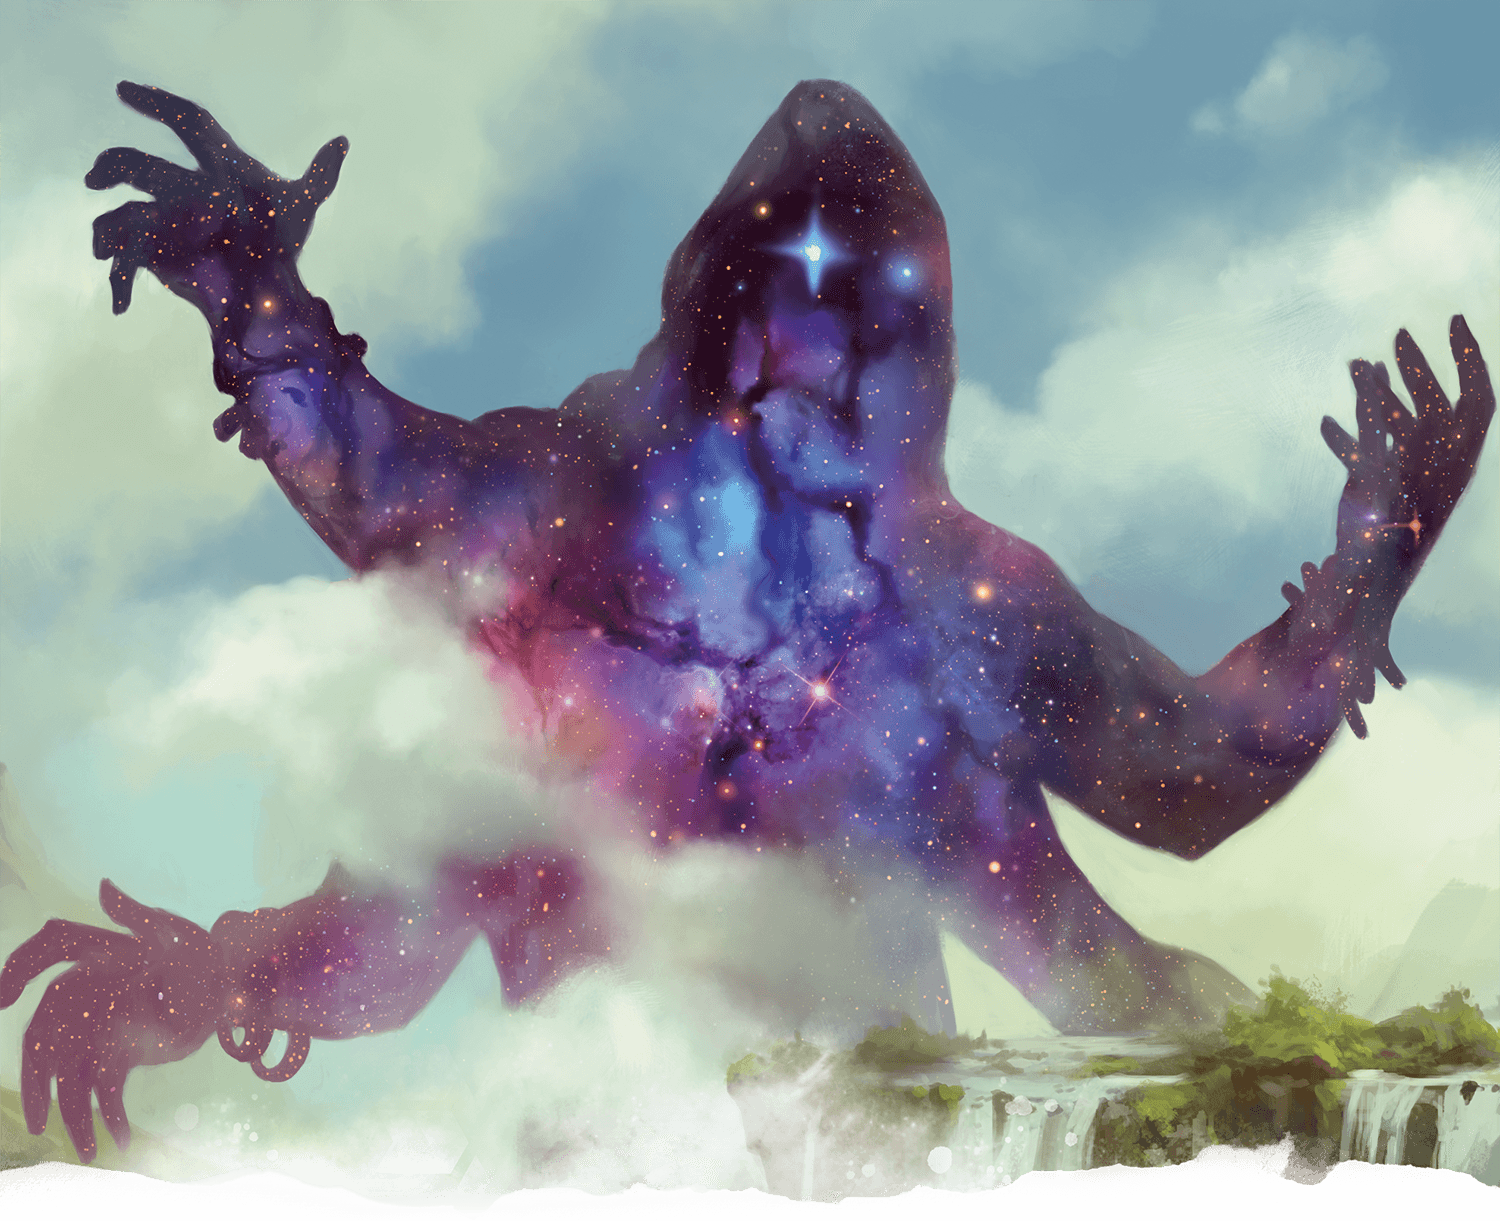
\includegraphics[width=\pdfpagewidth]{02viphoger/img/10kruphix.png}};
% \end{tikzpicture}
%
% \vspace{15.0cm}

\subsection*{Thassa, God of the Sea} \label{ssec::thassa}
    \subparagraph{Domains} Blue.

    Thassa is the god of the sea, aquatic creatures, and the unknown depths.
    She also holds sway over less tangible concepts such as ancient knowledge, long voyages, and gradual change.

    % Impassive and slow to anger, Thassa is secure in the knowledge that there are no mortals and few gods who can threaten her status.
    % Once her ire is aroused, however, it is as unstoppable as a cresting wave.
    % She often speaks in the future tense, referring to what tomorrow will bring.
    % She seldom laughs, and when she does, it is usually out of smugness rather than genuine mirth.

    Thassa usually appears to mortals in the form of a female tortle-like being with octopus-tentacle hair and a crown of crab legs.
    % She seldom adopts the same size as her followers, preferring to be seen from a distance as she towers over the ocean.
    When she moves close to the view of mortals, she takes many other forms, often shifting from one to another: a giant squid, an ocean storm, a school of sharks, a fog bank, or a crab, her favored animal.
    % She sometimes speaks out of the ocean itself, in droplets hissing across the surface of the waves.

    % \begin{figure}[b]
    %     \centering
    %     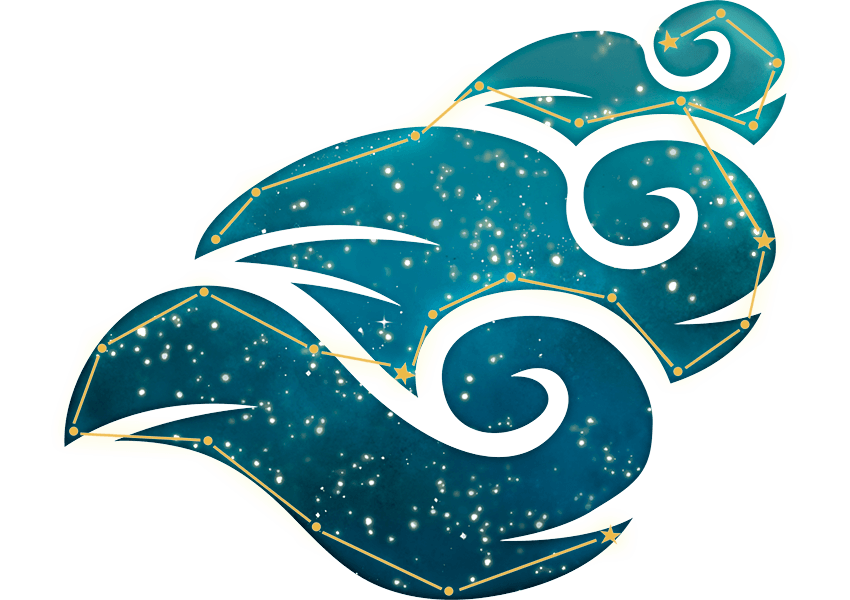
\includegraphics[width=0.47\textwidth]{02viphoger/img/10s_thassa.png}
    % \end{figure}

    \subsubsection{Worshiping Thassa}
        Most of Thassa's dedicated worshipers are tortles.% , and the vast majority of tortles are wholly devoted to Thassa.
        Tortles spend much of their lives in Thassa's realm, with their god omnipresent.
        They weave prayers to Thassa into nearly everything they do.

        Among the poleis, Thassa is worshiped by those who rely on bountiful seas for sustenance or calm waters for safety.
        Sailors, fishers, and residents of Viphoger's coasts and islands all pay her at least nominal respect and sacrifice.

        % Her center of worship on land is in the coastal polis of Mephetis, where sailors and philosophers pray to her for guidance.
        % The week-long Lyokymion festival (the Feast of the Melting Swell) marks the start of the new year by celebrating the bounty of the sea.

        % Thassa's most fervent gat worshipers offer prayers at high and low tide.
        % If possible, they do so at the water's edge.
        % At low tide they walk barefoot out onto the tidal flats, relishing the touch of Thassa's seabed.

\newpage

% !TEX root = ../main.tex
\subsection*{Piety \& Boons} \label{ssec::pietyandboons}
Being a god's champion carries no benefits in and of itself.
The gods do reward the devotion of their champions, though.
The strength of your devotion to your god is measured by your piety score.
As you increase that score, you gain blessings from your god.

Piety has nothing to do with faith or belief, except insofar as a person's thoughts and ideals drive them to action in a god's service.
Your piety score reflects the actions you have taken in your god's service --- actions that the god richly rewards.

When you choose a god to worship, your piety score related to that god is 0.
Your piety score increases by 1 when you do something to advance the god's interests or behave in accordance with the god's ideals.
The gods expect great deeds from their champions, so your piety score typically increases only when you accomplish a significant goal, make a significant sacrifice of your own self-interest, or otherwise when the DM sees fit.

The gods bestow favors on those who prove their devotion.
When your piety score crosses certain thresholds --- 3, 10, 25, and 50 --- you gain a benefit detailed in this section of your choice.
If your piety score exceeds and then falls below one of those thresholds, you lose the benefit you gained at the higher tier.

\subsubsection{Piety 3+}
    \subparagraph{Agonizing Strikes}
        You can add your Wisdom modifier to the damage of an attack.
        You can use this feature a number of times equal to your Wisdom modifier.
        You regain all expended uses of this feature when you finish a short rest.
    \subparagraph{Beast Speech}
        You can comprehend and verbally communicate with any creature with an Intelligence score of 5 or less.
    \subparagraph{Godly Influence}
        Your proficiency level in Persuasion and Deception is increased by 1.
    \subparagraph{Hero's Vigor}
        You gain 1d4 + 4 temporary hit points after you finish a short rest.
    \subparagraph{Nyx's Shield}
        While you're not wearing an armor, your AC is 12 + your Dexterity modifier.
        You can use a shield and retain this benefit.
    \subparagraph{Pact Weapon}
        During a long rest, you mark a weapon of your choice as a symbol to your god.
        That weapon is infused with your god's power, gaining a +1 bonus to attack and damage rolls for you until you finish a long rest.
    \subparagraph{Unyielding Sight}
        You can see in darkness to a distance of 24 meters.

\pagebreak

\subsubsection{Piety 10+}
    \subparagraph{A God's Gaze}
        Once per short rest, you can use an action to see through solid objects and darkness up to a range of 6 meters.
        This effect lasts for a minute.
    \subparagraph{Fagalian Cloak}
        Once per short rest, you can activate a godly aura to a radius of 1-meter around yourself as an action.
        You gain advantage on Intimidation checks while the aura is active, and all unfriendly creatures in the aura take necrotic damage equal to your Wisdom modifier (minimum of 1) at the start of their turns.
        This effect lasts for a minute or until you dismiss it as an action.
    \subparagraph{Freedom of Movement}
        You cannot be affected by difficult terrain, and your speed cannot be reduced except when you are restrained.
    \subparagraph{Godly Gift}
        You gain access to one spell with a spell point cost equal to 0.
        The spell is chosen by your DM, and pertains to your god.
    \subparagraph{Heavenly Protection}
        Once per short rest, you can negate all damage from one attack made against you as a reaction.
        You can use this ability after you know how much damage the attack would make.
    \subparagraph{Hero's Smite}
        All your successful melee attacks deal 1 force damage in addition to their normal damage.
    \subparagraph{Nyx's Veil}
        When you are in dim light or darkness, you can use two actions to become invisible.
        This invisibility remains until you take an action or reaction.

\subsubsection{Piety 25+}
    Your two boons are improved in a manner chosen by your DM.
    In addition, you can change one or both of your previously selected boons.

\subsubsection{Piety 50+}
    An ability score of your choice is increased by 2, as is your maximum for that score.
    In addition, you become a champion of your god, and they can grant you an artifact pertaining to them.

\newpage


% !TEX root = ../main.tex
\section{Akhosh} \label{sec::akhosh}
\DndDropCapLine{}{Only victory endures.}

\hspace*{\fill} --- Akhoash motto.

The walled polis of Akhosh stands defiantly atop a precipitous cliff.
The unforgiving Katajthon canyon under it serve as a shield between its holdings and the rest of Viphoger.
Few have ever dared to attack its famed fortress, the Kolophon, and no attack has ever breached its walls.
To the residents of Viphoger, the Akhoans hold near-mythical status: feared warriors produced by a culture that centers around perfecting the mind and body for war.
Their armies have rarely tasted defeat as they expand the borders of Akhosh, seizing new lands and bounty.

\subsection*{People of Akhosh} \label{ssec::peopleofakhosh}
    For most of Akhosh's neighbors, the term "Akhoash" evokes legendary warriors, trained from birth in every martial discipline known to gatkind.
    It brings to mind songs of tight-knit martial bands, holding strong in the face of unbeatable odds.
    It sings of a great yearly competition that crowns the preeminent warrior-athlete in Akhosh, and—by extension—Viphoger.
    The majority of Akhosh's inhabitants, though, aren't members of its martial elite.
    The famed warriors of Akhosh have the means to devote their lives to studying and training in the ways of war because they rest atop a rigid social structure of serfs and servants that largely dwell beyond the Kolophon's walls.
    % Those who stand at the heights of Akhoash society, or outside it, are detailed here.

    \subsubsection{The Monarchy}
        Traditionally, Akhosh is ruled by a gat monarch drawn from the lineage of lektoi.
        The monarchy passes from parent to eldest child, but any sibling or firstcousin of the heir can challenge this succession and claim the throne by besting the heir in single combat.

        Currently, the monarchy is in a state of turmoil.
        King Anax has died, and their child, Cymede, has disappeared.
        An oracle of Keranos, Cymede is said to have transformed into a pillar of fire and vanished into the wind, but until their death is certain, the lektoi are reluctant to name a new monarch.
        Anax has no other children, so the king's nephew, Taranika, acts as regent, attempting to guide the polis through what is sure to be a difficult transition.

        As if the situation weren't complicated enough, rumors have it that Anax isn't dead.
        They, or perhaps some shimmering simulacrum of him, has been seen at the head of squads of bughna gat hoplites, wielding an axe that billows with smoke and drips searing lava.

    \subsubsection{Lektoi}
        At the apex of Akhoash society are the lektoi, the large warrior class of Akhosh.
        Members of this class claim descent from the seven warriors who first established the Kolophon during the Sylvan wars.
        Though the families now number more than seven, each one uses an animal associated with one of the seven warriors as its symbol, either the ram, lion, horse, boar, badger, bull, or hart.
        The ram, associated with Akhosh's first king, Elektes, is commonly used as a symbol for the lektoi as a whole and for Akhoash strength, determination, and resilience.
        It is a popular theme in clothing, jewelry, and weapon ornamentation. % , and some lektoi even wear their hair braided into stylized ram horns.

        Although the lektoi claim descent from heroes, membership in this noble class isn't strictly hereditary.
        Anyone can earn a place among them by claiming a victory in the annual Iroan Games.
        More commonly, members of lektoi families lose their place of privilege if they fail to fulfill their obligation to serve in the Akhoash military.

    \subsubsection{Stratians}
        The Akhoash military is formed of wandering bands of warriors (drawn from the lektoi families) known as stratians.
        Outside the walls of the Kolophon, the stratians camp in the forests and fields, hunt game for food, and train younger warriors as they go.
        Their tasks are to search for creatures that have strayed into Akhoash territory and to protect travelers.

        Stratian forces are divided into three types of duty and armed appropriately for the task before them:

        \subparagraph{Alamon} Rugged forces of wanderers patrol Akhosh's borders, defending against invasion or attack by creatures that dwell in the mountains, foothills, and badlands around Akhoash territory.
        They are armed and armored for speed and agility, allowing them to move stealthily and strike unexpectedly.

        \subparagraph{Lukos} The most elite forces among the stratians, the so-called wolves contend with threats that the Alamon can't handle alone.
        After the guerrilla tactics of the Alamon have softened up a target, the heavily armored Lukos march to finish the task.

        \subparagraph{Oromai} The watchers are the guardians of the Kolophon who protect the fortress from invaders and maintain order within its walls.

    \subsubsection{Flamespeakers}
        Prominent spellcasters, the flamespeakers are reclusive priests of Purphoros who revere nature spirits and who inhabit fiery rifts in the mountains.

        \pagebreak

        % NOTE. At some point I should figure out how to use wrapfigure and tikzpicture together.
        \begin{tikzpicture}[remember picture,overlay]
            \node[anchor=north, yshift=0.10cm] at (current page.north) {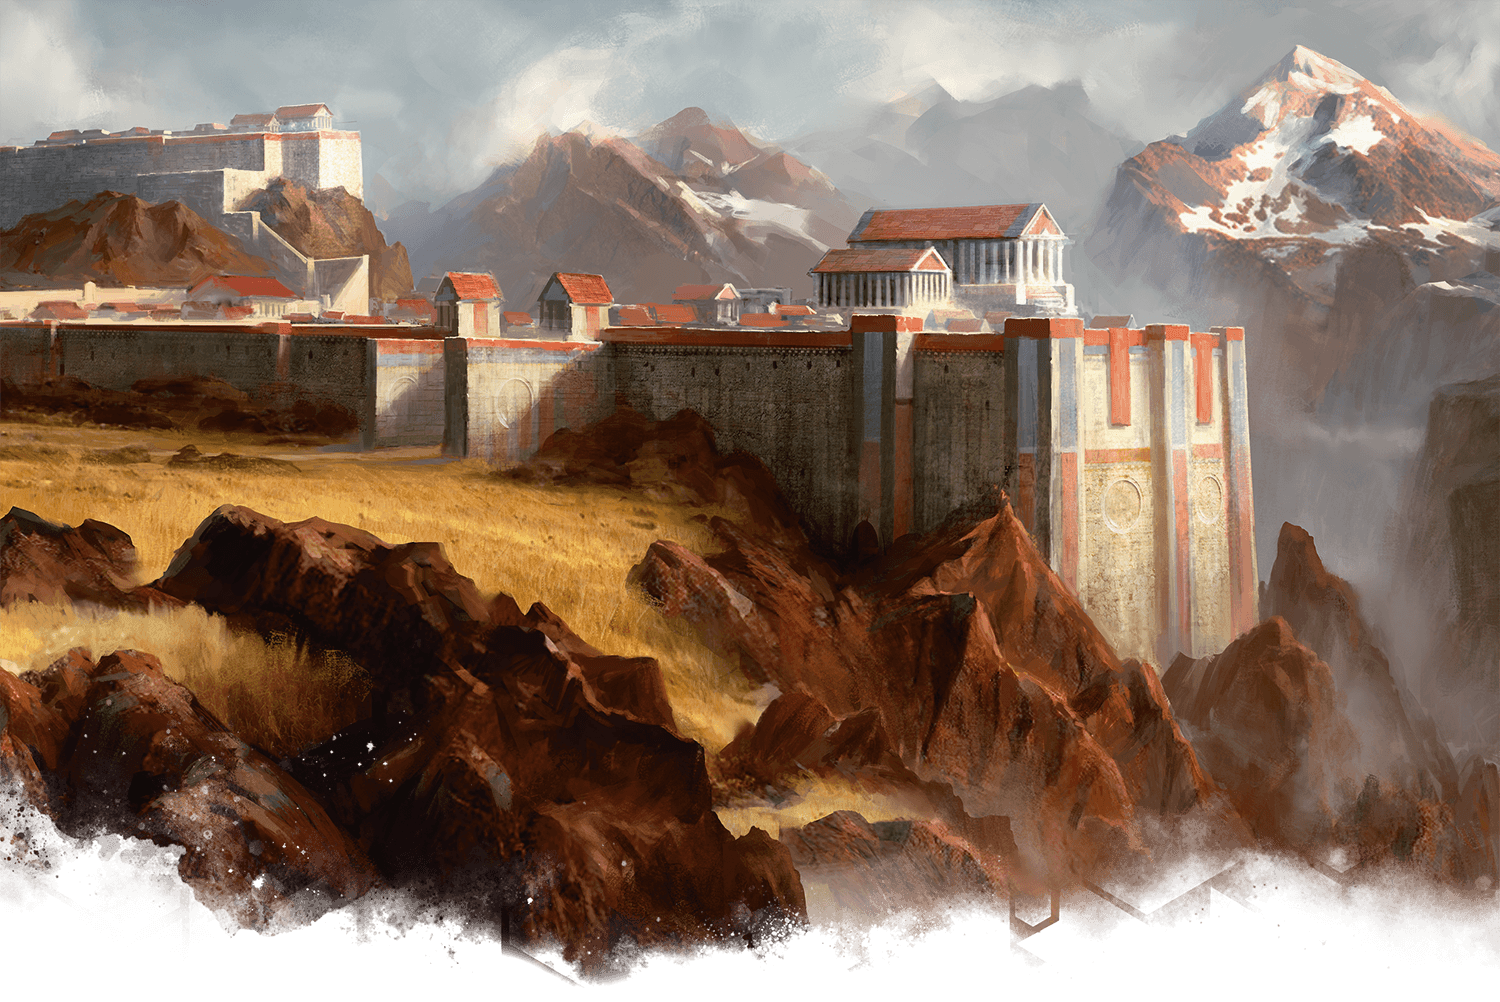
\includegraphics[width=\pdfpagewidth]{02viphoger/img/20kolophon.png}};
        \end{tikzpicture}

        \vspace{12.5cm}

        The ancient practice is viewed as primitive but powerful, and Akhoans of any background might risk making a pilgrimage into the mountains to hear a flamespeaker's prophecies.

    \subsubsection{Servants and Serfs}
        Lektoi who complete their military service with honor often retire to the Kolophon or their family estates and go about the leisured life of aristocrats.
        Their households are run by a class of servants made up of lektoi who were unable or unwilling to undertake a military career.
        These servants lack citizenship's full privileges but retain a position of some honor thanks to their class.

        Below these servants, at the bottom of Akhosh's social hierarchy, are the serfs.
        Comprising the vast majority of Akhosh's population, the serfs largely reside outside the protection of the Kolophon, laboring to grow the staple crops that support Akhosh's citizens and its trade.
        A relatively small number of serfs are skilled artisans who manage to build a more prosperous life for themselves with their crafts.
        But even these wealthier serfs can't own the land they live on, and they enjoy few rights or legal protections.

        \pagebreak~
        \vspace{12cm}

    \subsubsection{Nongats in Akhosh}
        Akhosh maintains a standoffish—and often hostile—stance toward its neighbors, particularly the treb gats of Phoberos, the leonin of Oreskos, and the dratl irds of the Pheres band.
        Members of those peoples rarely find a warm welcome in Akhoash territory.
        However, Akhoans respect prowess, loyalty, and self-sacrifice, and might welcome any who embody such virtues.
        Some stratians also seek to learn the martial practices of other peoples, and might invite individuals or small communities to Akhosh to learn their ways.

        During the Iroan Games, everyone is welcome in the stadium.
        Thousands flock to the city to witness the competition, and some take up permanent residence, celebrating the outcome of one year's games until it's time to start watching the next.

\subsection*{Features of Akhosh}
    At the center of the polis of Akhosh rises the Kolophon, a mighty fortress and the seat of Akhoash power.
    This many-tiered structure perches upon a vast cliff, which drops into a deep canyon carved by the Tsher River.
    Nature and Akhoash ingenuity conspire to make the Kolophon one of the most intimidating fortresses in Viphoger.

    \begin{tikzpicture}[remember picture,overlay]
        \node[anchor=north west, xshift=-0.10cm, yshift=0.10cm] at (current page.north west) {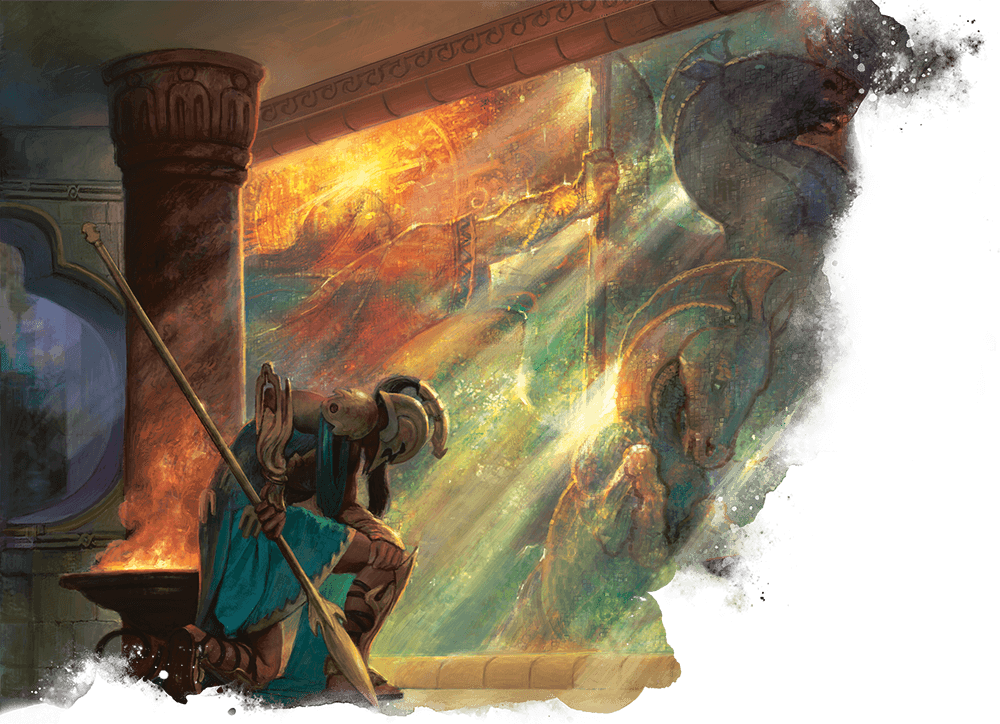
\includegraphics[width=0.5\pdfpagewidth]{02viphoger/img/20blessed_hoplite.png}};
    \end{tikzpicture}

    \vspace{6.2cm}

    Beyond the polis stretch craggy hills and canyon walls broken by narrow stretches of arable plains.
    It is a nearly impassable landscape, save for a few roads hewn through passes.
    Residents claim that only a fool would attempt to invade the heartlands of Akhosh, yet Akhoashs obsessively guard against invasion nonetheless.

    Beyond its thick walls, the streets of Akhosh are dotted with towering statues of heroes.
    Red-tiled roofs soar over square-topped sandstone columns, and holy sites dedicated to Iroas, Purphoros, and Keranos, among the other gods, are many.
    The architecture is formidable, spare, and militaristic, thick with sharp, angular shapes.

    \subsubsection{Temple of Triumph at Akhosh}
        At the heart of the walled city is the huge stadium that hosts Viphoger's greatest sporting event, the Iroan Games.
        A grand temple of Iroas stands beside it, serving as the venue for award ceremonies.
        A wide plaza connects the stadium to the city's outer gates, offering plenty of room for celebration around the annual games.

        When the stadium isn't hosting the actual Iroan Games, it is still used daily for training and for lesser athletic events.
        Many of the buildings surrounding the stadium are dedicated to serving it: smaller training facilities, providers of athletic gear, stables, and other shops.

    \subsubsection{Citadel}
        The uppermost tier of the city, perched on a rocky outcropping at the northwestern corner of the Kolophon, is the great citadel.
        The Oromai (the ``watchers'' who maintain order and defend the Kolophon) are quartered within the citadel's imposing walls, and the monarch's palace is built atop it.
        Temples of Iroas, Heliod, and Keranos also adorn the top of the citadel, the latter commissioned by the late prince Cymede, built with an open roof to give them a clear view of stormy skies.

\subsection*{Akhosh's Surroundings}
    Arable land is scattered across small plateaus and valleys in Akhosh, meaning that the serf communities that farm the land are small and just as scattered.
    Volcanic rifts, landslides, and venomous animals make travel dangerous for anyone who doesn't know the terrain, and visitors wishing to avoid suspicion from patrolling stratians would be wise to stick to the roads.

    \subsubsection{Outposts}
        The Alamon soldiers spend most of their time patrolling Akhosh's outlying areas, centering their patrols around scattered outposts.
        These serve as staging grounds for Alamon and Lukos units to prepare as they venture out to raid or guard against monsters and invaders.

        \subparagraph{One-Eyed Pass} The outpost in One-Eyed Pass serves to keep an Akhoash eye on the large cyclops population of the area, but the stratians also use the cyclopes to their advantage.
        Any time dangerous creatures come down from the mountains and pose a potential threat to Akhoash holdings, the Alamon harry the enemy and try to funnel them into the pass.
        The cyclopes of the pass viciously defend their territory against all intruders, weakening or even eliminating the danger before it can reach the Akhoash outpost, where the Lukos finish off any stragglers.

        \subparagraph{Pharagax Bridge} On the eastern border of Akhosh gapes a massive chasm rumored to descend all the way to Nyx and belch forth foul creatures.
        The great stone bridge that spans it is the only way into Akhosh from this direction.
        Stratians consider it a high honor to be assigned to guard the bridge.

        \subparagraph{Titan's Stairs} These stone ``stairs'', seemingly carved into the granite cliffs that protect Akhosh and haunted at all times by eerie, whistling winds, provide natural access to Akhosh.
        The stratians guard it fiercely and use it as a staging ground for invading the lowlands.

        \subparagraph{Katajthon Outposts} Several semipermanent encampments dot the rocky land between Akhosh and the rest of the Katajthon canyon.
        Fresh cadres of troops come here every month to relieve soldiers who are worn out by relentless assaults from raiders, fire-breathing dragons, and other threats.

        \subparagraph{Canyon Shrines} The Akhoashs believe that the gods are best worshiped at the places closest to the sky --- canyon peaks.
        Small temples and shrines are found throughout Akhoash territory.
        Some are tucked in caves or nestled in crevices or canyons, while others are bare altars exposed to the elements.

\subsection*{Pheres Lands}
    Between the dark polis of Kofos and the vast grasslands of Oreskos to the south, Pheres-band irds roam across the dry, hilly landscape.
    Gathered in small bands of fierce raiders, the Pheres irds plunder whatever prey they can find: merchants and other travelers moving between Akhosh and Setesh, settlers trying to eke out an existence in the region, leonin tribes, Vahagha-band irds who range too far to the south, and any others they encounter.

    The Pheres irds still follow the ways of the Hulnar empire, and these marauders take any opportunity to attack the Alamon.
    There have even been instances of direct attacks against Akhosh by the Pheres-band, where the quick and brutal tactics of the dratl irds are still able to catch off guard even the most elite of the Lukos.

\thispagestyle{empty} % Remove footer so that it doesn't clash with the image.
\begin{tikzpicture}[remember picture,overlay]
    \node[anchor=south, yshift=-0.10cm] at (current page.south) {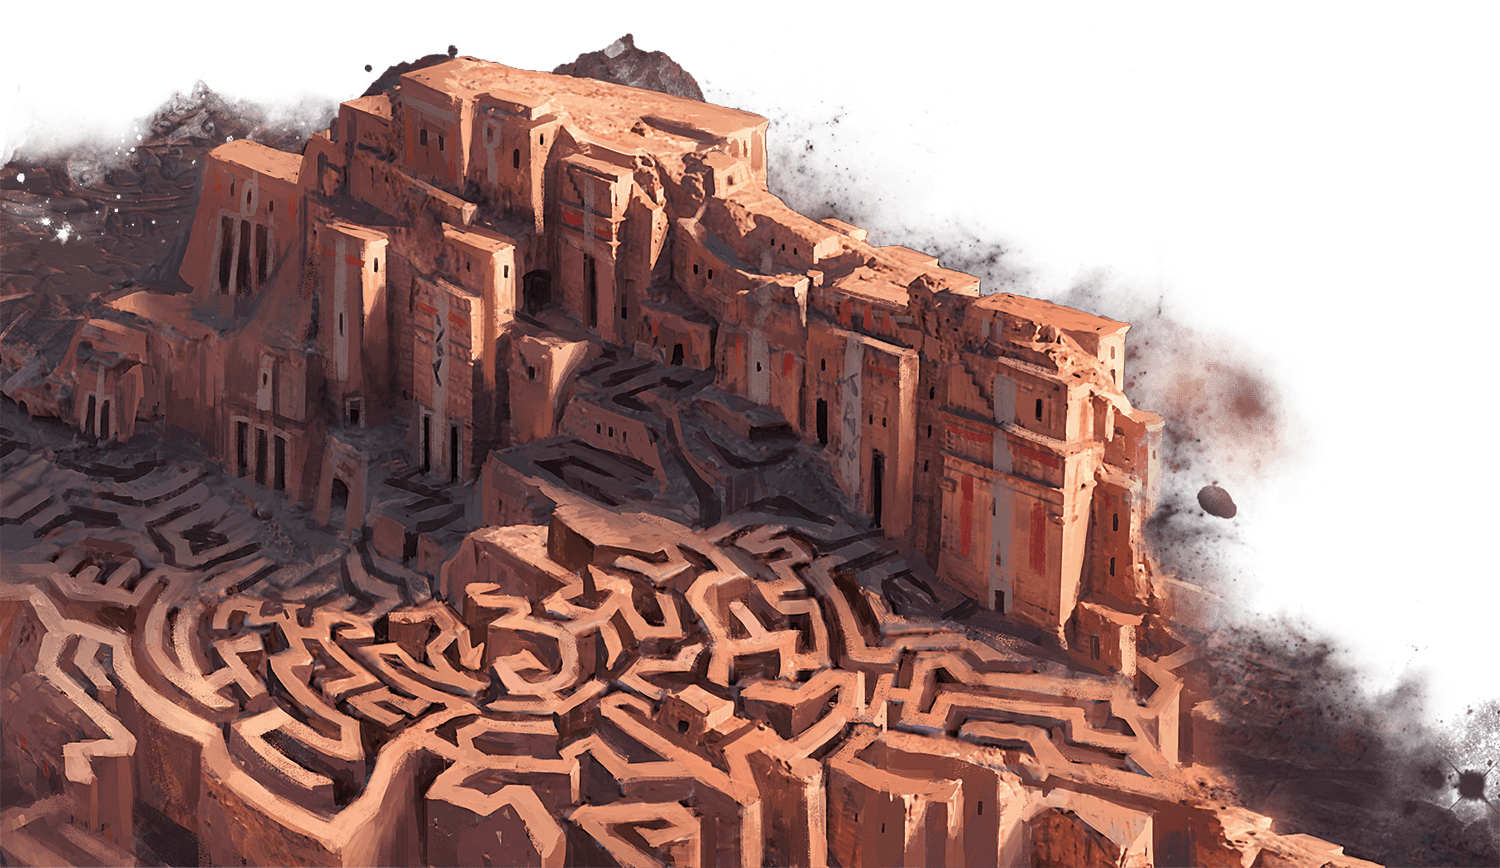
\includegraphics[width=\pdfpagewidth]{02viphoger/img/20kofos.png}};
\end{tikzpicture}

\subsection*{Kofos}
    The south-western edge of Akhoash territory is a region of arid canyons and caverns, a land of harsh natural whims haunted by ravenous monsters.
    Fierce bands of wild treb gats haunt these badlands, hailing from the Dead Sea to the east.

    At the southernmost point of this land, far from the walls of Akhosh, stands the sprawling, labyrinthine polis of Kofos.
    Kofos is mentioned in a few ancient odes, but only a handful of Viphogerians have ever beheld Kofos, and hardly any have successfully navigated its labyrinthine passageways and returned to tell of it.

    \newpage

    \begin{DndComment}[float=t]{Myth of the Akhoash War}
        Barely a year after the end of the Sylvan Wars, the Hulnar empire summoned the whole host of loyal spears from the house of Tadnas to wage war on the fortified canyon polis.

        What followed was a siege that stretched on for decades.
        Whole parts of Akhosh were destroyed and rebuilt in the fighting.
        There were heroes who knew only a life of conflict, performing feats of incredible prowess for the honor of Olantin, or who awed the gods with their sleepless commitment to defending the gates of Akhosh.

        Most people today know of the event from an embellished account laid down in an epic poem, The Akhoash War.
        Authored by the great poet Vefan, the poem is considered to be a definitive accounting of the greatest war in history.
        Countless soldiers aspire to fight with the honor and purpose that inspired the heroes of the Akhoash War.
    \end{DndComment}

    The founding of Kofos and its troubled history with Akhosh are the stuff of myth, and it is difficult to distinguish the mortal history of the two poleis from tales of the twin gods, Iroas and Mogis.
    The gods warred with each other, their followers and champions vied for control of scarce land, and two ideals --- the nobility of heroic struggle and victory versus the brutality of savage slaughter in war --- competed for a place in the mortal mind.
    Just as Mogis is the dark shadow of everything Iroas stands for, so is Kofos the reflection of Akhosh.
    And the shores of Tsher are the bloodstained battleground where the eternal conflict between the gods and their poleis is waged.

    Most of the treb gats that roam the upstream of the Tsher River are outcasts from the society of Kofos.
    They are bandits and marauders, bloodthirsty killers infected by the wild rage of Mogis.
    These gats have more in common with monsters than with the civilized people.
    Most of them use only the barest minimum of technology --- tattered clothes, piecemeal armor, and heavy weapons. % , all scavenged from their fallen foes.
    % They wander alone or gather in bands under the leadership of the strongest among them, and in either case tend to kill any person they encounter.
    % Three distinct bands are particularly well-known by their Akhoash foes: The Bloodhorn, the Felhide, and the Ragegore.
    % NOTE. Add all commented text if I ever manage to wrap text around these figures.

\newpage

% !TEX root = ../main.tex
\section{Mephetis} \label{sec::mephetis} % TODO: This section needs two more pictures. Get to it!
\DndDropCapLine{}{Evil flourishes where ignorance thrives.}

\hspace*{\fill} --- Perisophia the philosopher.

\thispagestyle{empty} % Remove footer so that it doesn't clash with the image.
\begin{tikzpicture}[remember picture,overlay]
    \node[anchor=south, yshift=-0.10cm] at (current page.south) {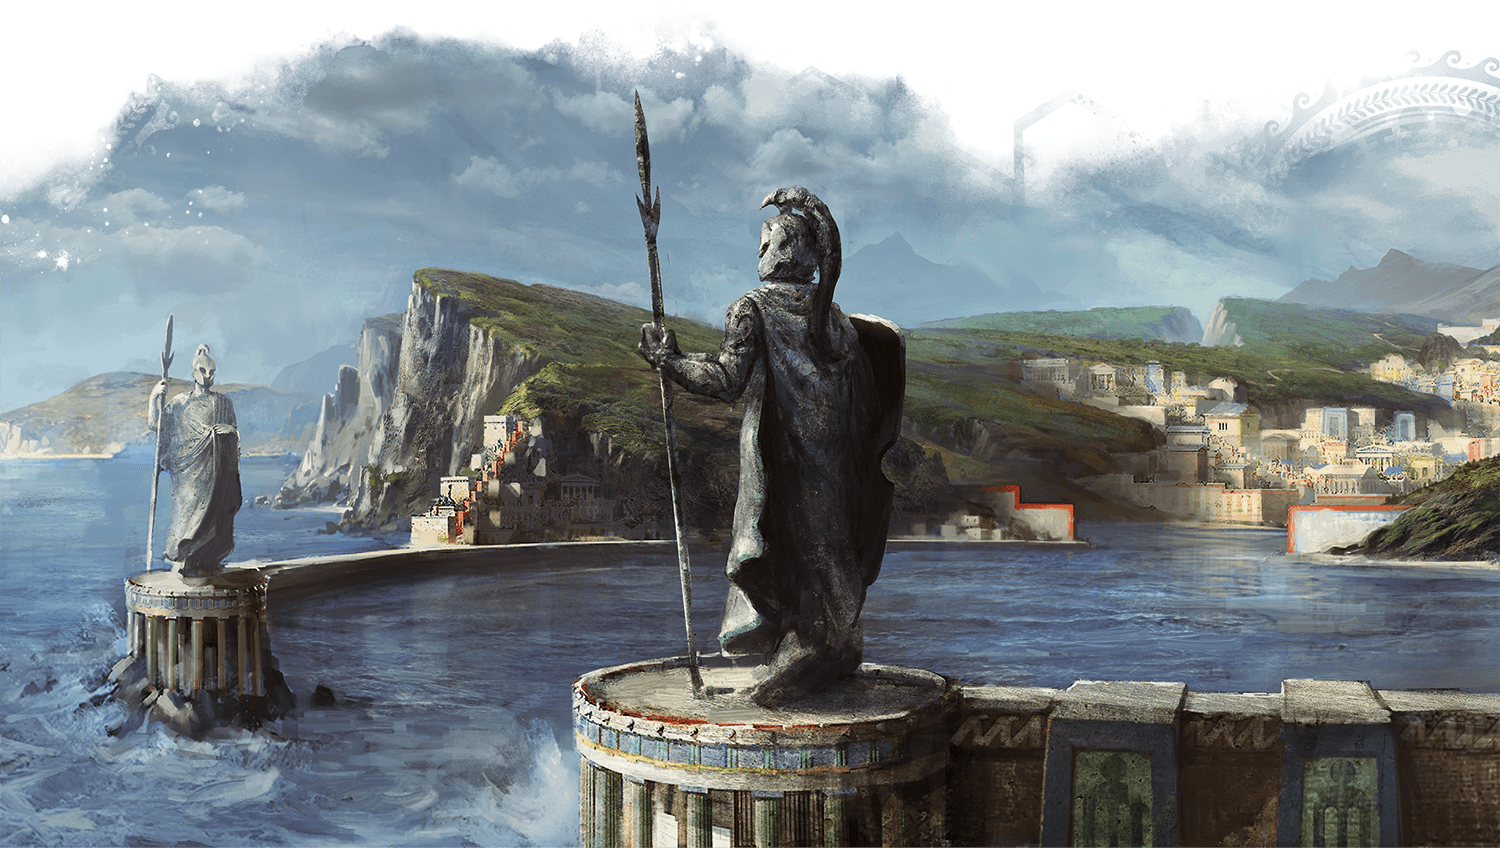
\includegraphics[width=\pdfpagewidth]{02viphoger/img/30seawall.png}};
\end{tikzpicture}

Mephetis is a polis devoted to learning, thaumaturgy, and progress.
It is the most populous city-state and home to progressive thinkers, pious thaumaturges, and wise oracles.
Born from the defeat of tyranny, to this day it pursues the ideals of free thought, societal betterment, and reinvention over stagnation and totalitarianism.

The et Agnomakhos ruled the area that is now Mephetis for centuries.
Impressing those they conquered into their legions, Agnomakhos aggressively expanded their kingdom, spreading it as far as the mountains to the south and the desert to the west.
Ultimately, though, the heroes Kynaios and Tiro overthrew the et.
From the kingdom's ruins rose Mephetis, a land that endeavors to reject cruelty and oppression throughout the world, and guards against hypocrisy within its own borders.

For a time, Kynaios and Tiro ruled Mephetis, striving to govern in accordance with the highest philosophical and ethical principles, which ultimately led them to relinquish their power and establish a philosopher-led republic.
After the kings' deaths, the council of scholars known as the Twelve took up rule of the polis, with the sage Elpidios serving as the senior member.

\newpage

\subsection*{People of Mephetis}
    The people of Mephetis take pride in their city's grand architecture, especially the great temples to the gods.
    They value philosophy and other intellectual pursuits, especially the practice of thaumaturgy.
    Mephetis's army is known for its discipline and its piety, and its navy is unparalleled.
    The city observes every one of the gods' holy days in various ways, and most residents try to live as the gods demand.

    Rich fields and the bounty of the sea support most people throughout Mephetis.
    The people have reputations for being accomplished weavers, skilled sailors, and cunning merchants.
    Books and literacy are also common throughout the land, and the work of scribes, cartographers, musicians, and storytellers is well regarded.
    The people of Mephetis believe themselves to be the inheritors of a heroic tradition, and each person owes it to themselves and to society to strive for greatness.
    Beyond Mephetis's common folk, a few groups that hold noteworthy standing are detailed here.

    \subsubsection{The Twelve}
        A council of philosophers called the Twelve serves as the ruling body of Mephetis.
        They are elected by popular vote among the citizens of Mephetis and serve for terms of four years at a time.
        They are supposed to govern by philosophical principles of justice and social order, and many of them do strive to uphold the highest ideals in their decisions.
        Others are more grimly realistic, and a few are deeply corrupt, serving only their own interests.

        \newpage

        The most senior member of the council is recognized as its leader, responsible for bringing the assembly to order and moderating its debate.
        Currently, this position is held by the renowned philosopher and orator named Perisophia.

    \subsubsection{Philosophers}
        Though they aren't necessarily heroic, philosophers are highly valued in Mephetis, which is renowned as the center of philosophical thought.
        They form a privileged class, often coming from wealthy families but also supported by stipends from the polis's academies and their own students.
        Different philosophical schools hold political as well as intellectual power in the polis, with five schools of philosophy dominating Mephetian discourse.

        \subparagraph{Elpidinas} Following the gold tide, Perisophia's optimistic Elpidian school currently predominates Mephetian thought and politics, carrying on the works of the heroic Epharan oracle Elpidios.
        The Elpidian school strives to put thaumaturgy and philosophy to use in improving the lives of all  Mephetians.
        Elpidian mages embrace magic in all its forms.

        \subparagraph{Formalists} Heralds of the indigo tide, formalist philosophers believe in a realm populated by abstract entities such as numbers and theories.
        They focus their efforts on trying to improve the moral fabric of the polis, hoping to create the ideal society, where people live together in peace, and where war and crime disappear.

        \subparagraph{Uremideans} Scholars of the blue tide, this school emphasizes logical reasoning, rhetorical excellence, and theories of ethics and virtue.
        Uremideans are eminently practical governors who seek to balance ethical ideals and realistic necessities.

        \subparagraph{Nykleans} Acolytes of no tide, nyklean philosophers teach that reason or destiny underlies all of reality, so that everything that takes place must unfold just as it does.
        These philosophers train themselves to accept and endure whatever befalls them, enjoying good fortune but not grieving its loss.

        \subparagraph{Anapsians} Followers of the red tide, anapsian philosophy embraces the fine delights of life: the pleasures of love and friendship, fine food and drink, art and music.
        Anapsians have few strong opinions about governance, except that an ultimate good end should be kept front of mind in all decision.

    \subsubsection{Thaumaturges}
        Mephetians view thaumaturgy as one of the greatest art forms, and they call the most accomplished mages thaumaturges or ``wonder workers''.
        Many Mephetian mages are trained at the elite academy of the Dekatia, but countless smaller schools and private tutors teach the magical arts.
        These lessons in thaumaturgy typically include a well-rounded education in the sciences and philosophy.
        Some thaumaturges find their magical studies aligning with popular Mephetian philosophies and choose the schools of magic they focus on based on such teachings.

        The mark of a true thaumaturge, though, is a gift or positive omen from the gods; even the most accomplished student of thaumaturgy can't earn the title without such a sign of divine approval.
        One mage might receive the gift of a spear from Heliod, another could receive a clockwork owl from Ephara, and still another might experience a wild, creative vision from Keranos.

    \subsubsection{The Reverent Army}
        The hoplites of Mephetis practice battlefield tactics in an environment saturated with religious devotion.
        The military force of the polis is called the Reverent Army, and aims as much to exalt the glory of the pantheon as to defend Mephetis.
        The soldiers are clever and resourceful, believing their piety leads the gods to smile upon them.
        More likely, though, their extensive training in battlefield tactics and thaumaturgy gives them an edge over other soldiers, with most Mephetian hoplites knowing at least a little magic.

    \subsubsection{Nongats in Mephetis}
        Mephetis strives to be a beacon to all of Viphoger's people.
        Well-intentioned members of any culture are welcome on Mephetis's streets, and the polis's people work to earn the trust of their neighbors.

        Of all the poleis, Mephetis has the closest relationship with the tortles of the Siren Inlet.
        Several communities of tortles consider the harbors of Mephetis and secluded coastal sanctuaries their home.
        Many take part in work near and under the water that other peoples are ill-suited to, but increasingly tortles find work not related to the sea, with tortle restaurants, chemists, and members of the Reverent Army being increasingly common.

        Mephetis maintains a fragile peace with the irds of the Vahagha band, engaging in regular trade.
        It's not uncommon for small groups of dral irds to set up shop in the polis market for short periods, though few spend more than a night or two in the city, most finding it claustrophobic at best.

        Few leonin journey to Mephetis, knowing little of the land beyond what their stories remember of Agnomakhos's tyranny.
        Even an age after the et's rule, most leonin view Mephetis as a cursed place.
        Those few who have traveled to the polis in recent years find it changed, with great potential for trade and cooperation, but no Mephetian or leonin has yet initiated an official dialogue between the two peoples.

        Most bughna gats have little patience for Mephetian philosophy, visiting largely out of curiosity or on elaborate larks.
        treb gats are rarely seen in Mephetis, though those who visit with peaceful intentions are welcome.

\subsection*{Features of Mephetis}
    The architectural and academic marvels of Mephetis testify to the achievements of civilized gats.
    The streets are paved with bricks made in interlocking geometric shapes, meant to demonstrate principles of both mathematics and thaumaturgy.
    Grand temples line the streets, testifying to the Mephetians' devotion to the gods.
    These rise as both mighty bastions dedicated to individual deities and various neighborhood shrines devoted to the pantheon as a whole.

    Inside the city, the wild lands feel like a remote threat.
    Perils from the sea present more obvious dangers, but a great sea wall protects the polis's port on the bay, while a lengthy channel cuts through the surrounding land to reach Mephetis Bay from the Whaler's Sea.

    \subsubsection{Pyrgnos}
        Many Mephetians speak of the ``edifice of knowledge'', referring in the abstract to the sum of all learning and scholarship.
        Every citizen is expected to help improving this edifice for the good of the polis, whether through philosophical exploration, advancements in magical technique, investigation into the nature of the gods, or perfection of techniques in crafting and trade.

        But the edifice of knowledge in Mephetis is a literal structure as well as a metaphorical one: the Pyrgnos is a glowing stone tower standing near the coast.
        It is literally formed from the collected learnings of the polis, recorded on carved stone tablets.
        At night, the top of the Pyrgnos shines like a lighthouse where the sea wall meets the shore, gleaming on the waters of the Siren Sea.

        A decade ago, the Pyrgnos was partly demolished by a kraken that attacked the city, but it has been repaired and continues to grow, reflecting the continued learning of the polis's citizens.

    \subsubsection{The Dekatia}
        Mephetis boasts many centers of learning, but the preeminent academy for philosophers and mages is the Dekatia.
        Students who display remarkable promise over the course of their earlier education can go on to spend up to ten years in arduous training at the Dekatia, apprenticed to master priests, thaumaturges, philosophers, and military heroes.
        Those who manage to complete this decade of training are renowned as the wisest of the wise and the bravest of the brave, combining all the essential learning of the polis into one package.

    \subsubsection{The Observatory}
        The Observatory is a tall viewing platform and a windowed structure offering a splendid view of the sky, renowned as a place to study the cosmos.
        Special crystals shaped by thaumaturges and blessed by the oracles of the gods enhance the view, making it easier for observers to see the workings of the gods among the stars and constellations.
        Priests, mages, and philosophers interpret what they see in the Observatory as signs and omens from the gods.

\subsection*{Mephetis's Surroundings}
    Mephetis sits on the coast of the Whaler's Sea, surrounded by rivers, sparse woodlands, and vast, stepped grasslands.
    Fields of barley provide sustenance to Mephetians and their animals.
    Well-trod roads wind their way through the region, but most locals travel along the coast in simple boats.

    \subsubsection{Mephetian Holdings}
        The polis of Mephetis embodies the heart and mind of what it means to be Mephetian, but the polis's lands also includes numerous other settlements and wildernesses.
        The people who live in these holdings are no less Mephetians than the inhabitants of the city, and they share the values of other Mephetians even if their lifestyle affords them little opportunity to study magic and philosophy.

        \subparagraph{Avtrisos} This small walled city is famous for Ephara's intervention to protect it from an illhevi, their face coming to life on the marble wall and making the barrier grow so tall that the illhevi couldn't get through.
        Avtrisos now has Ephara's face on nearly every building and wall in the entire city in gratitude.

        \subparagraph{Bjokesh} Bjokesh is a small coastal town that would be completely unremarkable, except that it's accumulated a truly impressive library.
        The bulk of the town's economy revolves around maintaining the library and meeting the needs of travelers who come to visit it.

        \subparagraph{Krinnos} Renowned as the home of Anapse, the ird philosopher who founded the Anapsian school, the village of Krinnos attracts many philosophers who share Anapse's delight in the pleasures of a simple life.

        \subparagraph{Listes} Listes is a fortress marking the southwestern border of the polis.
        The civilian population is hardly less disciplined than the members of the Reverent Army stationed there, and the whole population observes Iroas's holy days together.

        \subparagraph{Natumas} The residents of Natumas are famous for training sea animals as skillfully as Seteshans train land and air animals.
        They train sea snakes, dolphins, and even sharks on a few occasions to be combatants, working animals, aquatic mounts, and companions.

        \subparagraph{Neshantin} Though they are regarded as Mephetians, the people of Neshantin view themselves as citizens of Olantin --- a coastal polis that long ago vanished into the sea.
        According to legend, an angry Heliod smote the polis with their spear, sinking it in punishment for its people's utter hubris.
        The fact that the Neolantians were spared this fate, they say, is evidence of their humility, and they take special care in their sacrifices to Heliod.

        \subparagraph{Oxus} Oxus is a quiet town with a notably wealthy population, consisting largely of merchants who have retired from trade with large fortunes at their disposal.
        The tomb of Kynaios and Tiro also stands in the center of the town, the subject of many local legends.

        \subparagraph{Phratsh} A small fishing village, Phratsh is most noted as being the literal "end of the road" for travelers venturing south from Mephetis.
        The rugged lands beyond are rocky and scattered with forgotten ruins.

        \subparagraph{Sitrum} This coastal town is known for the way many of its buildings are on stilts to accommodate the changing tides.
        Sitrum is famed for its skilled shipwrights.

        \subparagraph{Thestre} The village of Thestre is little more than a crossroads, but it's notable for its temple to Karametra.
        The site draws farmers from the region who offer a portion of their crops to the god of agriculture.

\newpage~\pagebreak % TODO: Add more stuff here.

% !TEX root = ../main.tex
\section{Setesh} \label{sec::setesh}
\DndDropCapLine{}{This city saved me when I was an}
\textit{orphaned child, sold into chains.
Now is my turn to save it.}

\hspace*{\fill} --- Kallias, Ophis Tower commander

Setesh is the favored polis of Karametra, and its buildings blend so perfectly into the forest that it's difficult to tell the difference between inside and outside.
The populace lives in harmony with the thick forests, terraced farms, and trained animals of Setesh, and they celebrate the cycle of seasons with grand holidays.

Setesh is also unique among the poleis of Viphoger in that few of its adult residents are gats.
Umans comprise the bulk of the population, holding almost all of the leadership roles and carrying out most work.
Gats are few and far between, and the other kins are even rarer in the polis.

The Seven Kingdoms of the Sea hold an intolerant attitude toward umans, where they are sold as slaves on most ports.
In Khedrat this situation is even more dire, where king Olag ordered the execution of all umans.
The ones that could escaped, and founded Setesh; hidden by the thick Nessian Wood.

% Children run freely around the polis.
% They're so important, in fact, that Setesh's people take in abandoned children from all over Viphoger.

\subsection*{People of Setesh}
    The populace of Setesh live in a beautiful paradise, and they're prepared to fight to the death to protect it.
    The constant training in archery, falconry, riding, and close combat can seem out of place among the idyllic forests and beautiful gardens and orchards, but that is the way of life in Setesh.

    \subsubsection{Gender in Setesh}
        Seteshans believe that women become heroes through martial exploits, while men do so by finding their own way in the world.
        As a result, the polis is populated mostly by women and children.

        When young men reach the age of fourteen, their rites of passage culminate in a journey called peregrination, where they wander the land until they find a new place to call home.
        The few men who reside permanently in Setesh live in the Amatrophon, training and caring for the animals there.
        Some of these men never peregrinated, but others left and then returned to Setesh.

        The women of the polis form a tight-knit community where property is held in common.
        There is no marriage, and ancestry is traced matrilineally.

        Despite the very different roles played by men and women, Seteshans are flexible when it comes to any individual's place in that structure.
        Some men set out on peregrination after spending a number of years identified as women, and some women return from peregrination (or never undertake it) after a period of realization.
        Some people move fluidly between roles, and a few choose a special role that Seteshans view as standing outside the dichotomy of gender, living in Ophis Tower.

        The warriors of Ophis Tower are martially trained as women are but wander the world as men do.
        They gather information for the Ruling Council, search out routes for peregrination (including identifying sympathetic individuals and households who will mentor young men at the start of their journeys), and rescue lost and abandoned children from other communities, bringing them back to Setesh.

    \subsubsection{The Ruling Council}
        Karametra is the queen of Setesh, but of course gods have more important concerns than the day-to-day governance of a uman polis.
        So a five-member council attends to the daily tasks of leadership on the deity's behalf.
        The council is made up of the commanders of the four prominent fortress-watchtowers that guard the polis.
        These commanders are elected by popular vote: Anthousa of Leina Tower, Phaedra of Hyrax Tower, Niketa of Bassara Tower, and Kallias of Ophis Tower.
        The fifth member is Silverbrow, a dratl ird oracle who reads the Kelema Veil at the Nexuses of the Seasons and advises action based on her visions.
        Anthousa is the head of the council, considered Karametra's closest advisor and the de facto ruler of the city.

    \subsubsection{Defenders and the Four Towers}
        Karametra includes defense of the home in her domains, and the residents of Setesh follow suit.
        Seteshan military forces are organized into four major regiments, each associated with a fortress tower.

        \subparagraph{Bassara Tower} The tower of the fox stands near the Summer Nexus and watches for interlopers who enter the Nessian Wood without permission.
        During their training, troops there focus on archery and guerrilla tactics.
        Their leader is Niketa, a woman in her fifties who spends most of her time in the tower since she parted ways with her partner.

        \subparagraph{Hyrax Tower} The tower of the falcon lies on the ridge near the Winter Nexus.
        Its regiment includes contingents of scouts and falconers.
        Its leader is Phaedra, a nineteen-year-old master falconer and orphan from Mephetis who was rescued by the Ophis regiment.

        \subparagraph{Leina Tower} The tower of the lion stands near Karametra's temple at the heart of Setesh.
        Its regiment, led by the hero Anthousa, is dedicated to the defense of the polis and the training of its children.
        The Leina warriors favor double-edged axes.

        \subparagraph{Ophis Tower} The tower of the serpent nestles at the center of Setesh.
        Its wandering warriors travel the world, working on behalf of the Ruling Council.
        Their leader is Kallias, who was sold into slavery as a child.
        They lost an eye and several fingers before they were rescued and brought to Setesh, where they have devoted themselves to saving others in a similar plight.

    \subsubsection{The ``Little Bears'' of Setesh}
        Children in Setesh are reared by the polis as a whole and treated with the highest respect; their welfare is paramount and their training is a significant part of every warrior's occupation.
        Orphans and abandoned children are sacred to Karametra, so they are brought into the city and tended just as Setesh's own children are.

        In contrast to the discipline associated with educating children in other poleis, Seteshan youngsters enjoy tremendous freedom.
        Called arkulli, meaning ``little bears'', they are welcome anywhere in the city.
        They often wander in and out of the temple, training grounds, the hall of the Ruling Council, the market, and anywhere else their paths take them.
        Such freedom is meant to cultivate a curious spirit and help the children find the path they're most interested in following later in life.

    \subsubsection{Nonumans in Setesh}
        Setesh doesn't welcome outsiders, as a rule, except the orphaned and abandoned children brought to live in the polis.
        But the polis can be more hospitable to nonuman outsiders than to umans (especially male umans) from other poleis.
        A few irds of the Vahagha band, leonin, and treb gats have earned the right to live in Setesh.
        Dryads and naiads from the Nessian Wood rarely try to enter the polis, but they are often friendly with the Bassara soldiers who patrol the forest.

\subsection*{Features of Setesh}
    Setesh fuses nature and civilization into a single living organism.
    The polis extends from a huge tree at its center, like the rings of a still larger tree.
    A dense circle of vegetation forms the city's outer wall, with the treetops woven together to create a barrier against intruders.
    Expertly trained archers stand guard on platforms nestled among the upper branches.
    Inside these natural walls, patches of thick forest alternate with open spaces where the Seteshans build their homes and civic buildings amid the trees.
    Out of deference to Nylea, the residents of Setesh never construct a building that isn't absolutely necessary, and their homes and buildings are seamlessly integrated into the environment, with vegetation weaving together into walls or roofs.

    \subsubsection{Temple to Karametra}
        In the very center of the city is the temple to Karametra, patron of Setesh.
        Three ancient trees grow from an earthen rise and spiral around the heart of the city.
        The temple, built of glittering limestone, nestles amid the massive trunks.
        Strong magical wards protect the temple, since Karametra herself sits here when she visits her beloved polis.
        All manner of civic functions are based in the temple, and most of them are carried out by Karametra's attendants.
        These attendants serve as healers, advisors, teachers, chroniclers, and oracles.

    \subsubsection{Nexuses of the Seasons}
        Four holy sites, corresponding to the four seasons, stand in or near the polis and serve as temples --- primarily for the rites of Karametra and Nylea, but also to the other gods to an extent.
        These nexus points between the mortal world and Cosmos --- a phenomenon called the Kelema Veil --- are where omens manifest amid star fields that glitter in the shadows and where oracles seek messages from the divine. The four nexuses are each distinct in their own ways.

        \subparagraph{Spring Nexus} Associated with Karametra, the Spring Nexus is located in a lavish garden just behind her temple in the city of Setesh.
        A large arch of vines and flowers leads into the nexus itself and stays fresh and green all year long.
        Spring is the most celebratory time for Seteshans --- a time for planting and hope.
        Worshipers leave gifts for both Karametra and Nylea here.

        \subparagraph{Summer Nexus} Located in an olive grove west of the city proper, the Summer Nexus is covered by a leafy green canopy.
        As a shelter from summer's heat, the nexus is a favorite resting spot for people and animals alike, and Nylea and Iroas are worshiped here.

        \subparagraph{Autumn Nexus} Near the southern edge of Setesh, in an orchard filled with golden apples, a small cave behind a basalt arch holds a perpetually burning flame.
        Priests keep a strict rotation to ensure the fire never goes out, as it represents Purphoros's fire that keeps the world warm through the colder seasons and allows the autumn harvest.
        In addition to Purphoros, Seteshans come here to worship Iroas and Mogis, when necessary.

        \pagebreak

        \begin{tikzpicture}[remember picture,overlay]
            \node[anchor=north, yshift=0.10cm] at (current page.north) {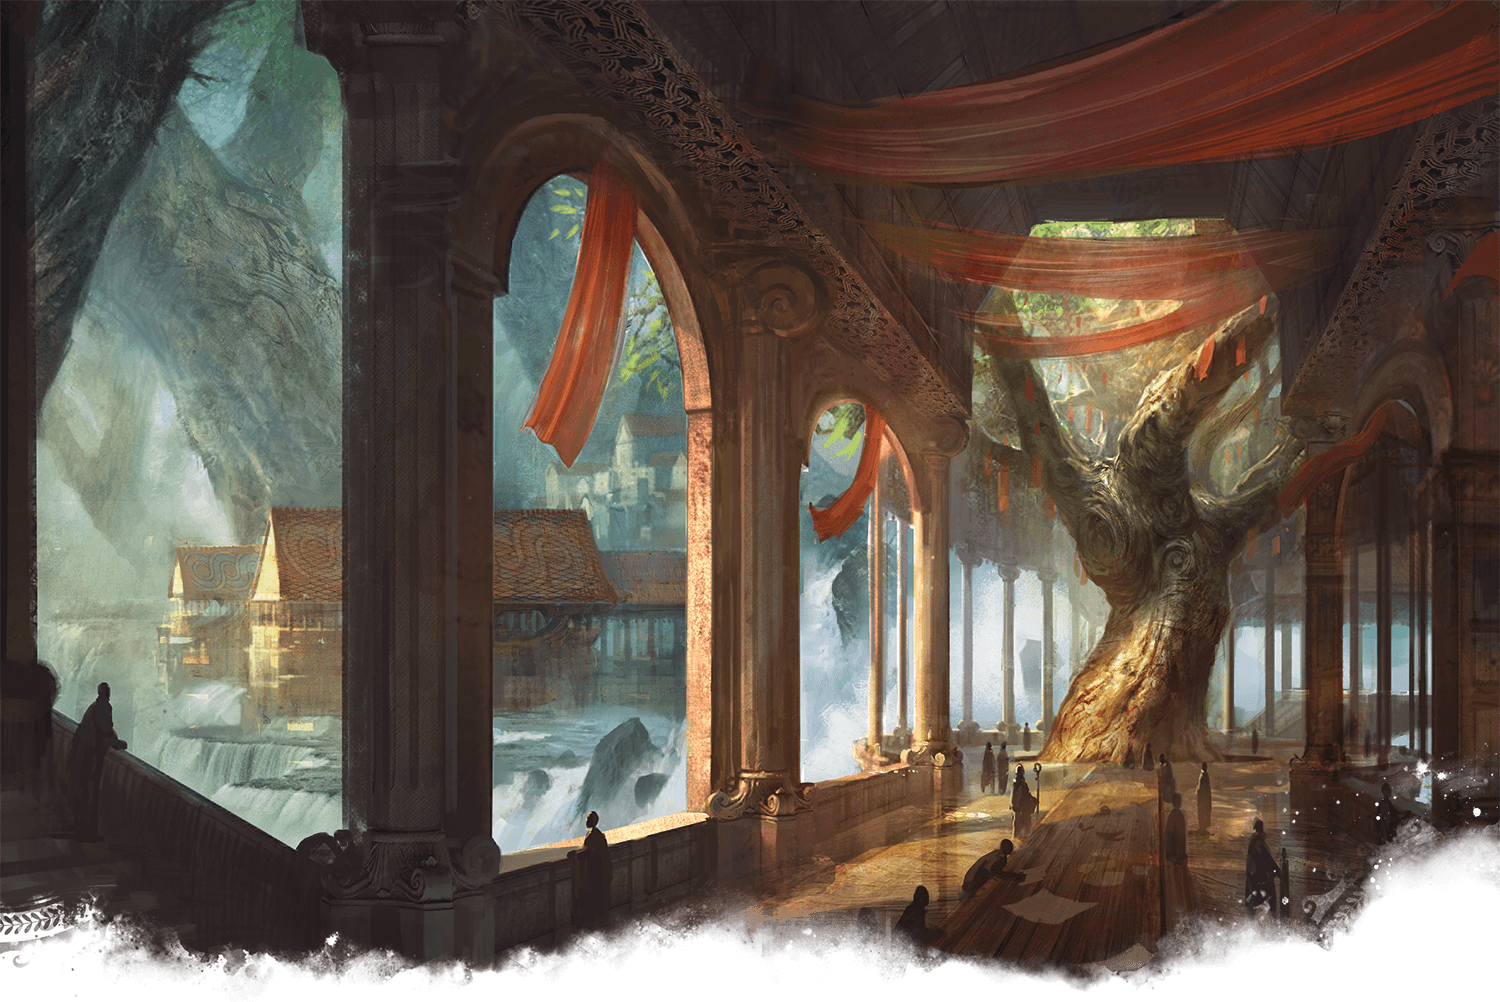
\includegraphics[width=\pdfpagewidth]{02viphoger/img/40setesh.png}};
        \end{tikzpicture}

        \vspace{12.5cm}

        \subparagraph{Winter Nexus} At the eastern edge of Setesh hides a rocky cave that was once a lion's den.
        The cave contains a burial ground and is rumored to lead all the way into the underworld.
        Seteshan children occasionally dare each other to see who can make it the farthest into the cave, but the morbid atmosphere usually sends the children scurrying back before long.
        Seteshans come here to worship Pharika and Erebos, paying respects to the dead or hoping to fend off death for a while yet.

    \subsubsection{Abora Market}
        The Abora Market is a giant, open-air market just inside the main eastern gate of Setesh.
        Every day it is thronged with citizens buying and selling food, crafts, and curiosities.
        On the seven days surrounding the full moon Fagal, outsiders are even allowed into the market, though they are still prohibited from roaming the rest of the polis.
        Visitors who try to explore beyond the market are typically banned from the polis and must forfeit any goods they brought into the city.

        The most impressive part of the market is the raptor hall, where falconers show off the trained raptors available for sale.
        Hunters all over the Viphoger come to buy famous Seteshan falcons.

        \pagebreak~
        \vspace{12.5cm}

    \subsubsection{Caryatid Groves}
        Scattered throughout the city are several groves that are sacred to Karametra and Nylea, made up of slender trees with almost umanlike forms.
        It is said that whoever enters one of these sacred groves in search of peace will find it --- and take root, becoming part of the grove.
        % NOTE: For the stats of the caryatids, use the Animated Tree.
        The trees here are caryatids, capable of animating in defense of the groves or the city but otherwise resting in silent stillness.

\subsection*{Setesh's Surroundings}
    Beyond the city's encircling trees, the territory of Setesh extends to cover about a third of the Nessian Wood and a wide swath of the open chaparral.
    In contrast to Mephetis and Akhosh, no villages or military outposts mark Seteshan territory, but a few key features in the Nessian Wood define the area under Seteshan control.

    \subsubsection{Amatrophon}
        The Amatrophon encompasses a large forested region at the southwestern edge of Seteshan territory, and it provides a safe haven and training ground for the diverse range of animals that occupy an honored place as natural protectors in Seteshan society.
        Experts train the renowned falcons of Setesh here, along with horses for riding and for combat.
        More unusual animals are found here as well: trainers work with boars, wolves, and lions to get them ready to accompany Seteshans in battle.
        Here men live and work alongside women, collectively training and caring for the animals that live here.

    \subsubsection{Nessian Wood}
        The vast wilderness of the Nessian Wood is considered Nylea's domain.
        Its trees are as old as the world, twining together to form an impenetrable canopy shielding the wood from Heliod's angry glare.
        Their roots stretch deep into the earth, and some say they drink from the Rivers That Ring the World, the waters of the Underworld.
        All manner of wild and strange creatures dwell in the Nessian Wood, far from the reach of civilization.

        Nylea allows limited hunting in the Nessian Wood, but she has been known to kill those who poach without her permission.
        Setesh's Bassara regiment helps the god keep an eye out for such illicit hunters, as well as any intruders who might bring danger upon the polis.

        \subparagraph{Cypress Gates} A natural gap between the Oranad Mountains and the Phoberos Canyon on the west side of the Milakul Swamp provides access into the Nessian Wood from the west.
        Ancient umans carved an impenetrable fortress into the mountains to guard the pass.
        Bassara patrols from Setesh still check in on the fortress regularly, and they occupy the fortress when there is reason to suspect danger from the west.
        More than once, though, patrols have reached the fort only to find something else has taken up residence, whether it be rowdy irds, grim Returned, or worse.

        \subparagraph{Hunter's Crossing} Setesh once extended its claim over more of the forests, establishing military outposts like those of Akhosh.
        At the western end of the woodlands, along the road from Kofos known as the Guardian Way, the ruins of a round tower lie beside a rushing stream.
        This marks the greatest extent of ancient Setesh's reach.
        A site of rich natural beauty, with lilacs growing along the riverbank and silver fish darting in startlingly clear water, it is abandoned by Setesh and favored by travelers as a resting point on the road before coming under the eaves of the forest.

\begin{DndComment}[float=h]{Myth of Nikaia the First Caryatid}
    A Seteshan archer named Nikaia claimed that she could outshoot anyone, even Nylea.
    Word of this unwise boast spread, and in response Nylea appeared at the next archery contest at the Spring Nexus.
    She challenged Nikaia to an impossible feat of archery: to shoot an arrow into one of the twin trunks of Kruphix's great tree at the edge of the world.
    Nikaia immediately realized that neither refusal, failure, nor success would forestall Nylea's wrath.
    Nonetheless, she held her head high, she and Nylea both let fly, and both arrows hit.
    Impressed by the mortal, Nylea took Nikaia to her sacred grove and planted her there as a caryatid, immobile but forever occupying a place of honor.

    Since then, Nylea has honored dozens of other champions and worthy mortals, blessing them with the long lives of mighty trees.
    The grown seedlings of Nikaia and Nylea's other favored continue to share their wisdom and protect Setesh to this day.
\end{DndComment}

